%   MSc Business Analytics Dissertation
%
%   Title:     The Relationship Between Corporate Governance and Company Performance
%   Author: Conor Reid 
%
%   Chapter 4: Results
%

\chapter{Results}\label{C.Results}

\section{Introduction}\label{S.intro4}
{As mentioned in previous chapters, there are three stages of analysis carried out as part of this study. The first revolves around replicating the work of \cite{moldovan2015learning}, who modelled the research question as a classification problem by thresholding on the continuous dependant variables measuring corporate success. The second stage neglects this thresholding leading to a regression analysis. The third takes the results of the first two and implements propensity score matching in an effort to infer causal influences to strengthen statements previous made based on correlations. This chapter outlines the results of each stage in turn.}
\section{Classification}\label{S.classification4}
%{\cite{moldovan2015learning}, for each of the three datasets, implemented four separate algorithms and used common performance metrics across all four to enable comparison. The four algorithms were all used for classification, namely Adaboost M1, J48, Simple Log and ADTree. This study takes both Adaboost M1 and an implementation of J48 and aims to replicate these results. We use similar measures of model performance. }
{As mentioned above, this study aims to replicate the results of the work of \cite{moldovan2015learning} using implementations of two of the classification algorithms used in that study. Similar performance measures are used to enable easier comparison.}

{Below are reproductions of \cite{moldovan2015learning} results.}\\

\subsection*{SPX}
\cite{moldovan2015learning}
\begin{table}[h!]
\centering
\begin{tabular}{ |p{2.5cm}|p{2cm}||p{2.5cm}|p{2cm}|p{2cm}|p{1cm}|  }
 \hline
 \multicolumn{6}{|c|}{Dependent Variable : Tobin's Q} \\
 \hline
 Algorithm & Study & Accuracy (\%) & Precision Class 0 & Precision Class 1 & ROC \\
 \hline
 Adaboost M1 & M\&M &  89.7177 & 0.89 &  0.905 & 0.957  \\
 Adaboost M1 & C & 93.3734  & 0.95 & 0.915  &  0.933 \\
  Adaboost M1 & C\textbackslash NO & 92.1213  & 0.948 & 0.897 &  0.922 \\
 & & & & & \\
 J48  & M\&M & 85.2823  & 0.841 &  0.866 & 0.854  \\
 J48  & C & 87.9518  & 0.840 & 0.930  & 0.885  \\
 J48 & C\textbackslash NO & 87.951  & 0.886 & 0.871  & 0.879  \\
 \hline
\end{tabular}
\caption{Classification Results - SPX, Tobin's Q}
\end{table}


\begin{table}[h]
%\centering
\begin{tabular}{ |p{2.5cm}|p{1.5cm}||p{2.5cm}|p{1.6cm}|p{1.6cm}|p{1.6cm}|p{1cm}|  }
 \hline
 \multicolumn{7}{|c|}{Dependent Variable : Altman Z Score} \\
 \hline
 Algorithm & Study & Accuracy (\%) & Precision Class 0 & Precision Class 1 & Precision Class 2 & ROC \\
 \hline
 Adaboost M1 & M\&M  &  82.944     & 0.843 &  0.725 & 0.865 & 0.942  \\
 Adaboost M1 & C & 84.892 & 0.818 & 0.529  & 0.910  & 0.861  \\
  Adaboost M1 & C\textbackslash NO & 83.3334 & 0.818 & 0.348  & 0.957 & 0.879  \\
  & & & & & &\\
 J48  & M\&M & 73.6086  & 0.722 &  0.569 & 0.816 & 0.843  \\
 J48 & C & 81.2949 & 0.591 & 0.529 & 0.910  &  0.832 \\
 J48 & C\textbackslash NO & 78.985 & 0.629 & 0.400  & 0.871 &  0.802 \\
 \hline
\end{tabular}
\caption{Classification Results  - SPX, Altman Z Score}
\end{table}







\clearpage
\subsection*{SXXP}
\begin{table}[h!]
\centering
\begin{tabular}{ |p{2.5cm}|p{2cm}||p{2.5cm}|p{2cm}|p{2cm}|p{1cm}|  }
 \hline
 \multicolumn{6}{|c|}{Dependent Variable : Tobin's Q} \\
 \hline
 Algorithm & Study & Accuracy (\%) & Precision Class 0 & Precision Class 1 & ROC \\
 \hline
  Adaboost M1  & M\&M &  88.2353     & 0.891 &  0.874 & 0.946  \\
 Adaboost M1 & C &  90.9547 & 0.904 & 0.916  & 0.910  \\
  Adaboost M1 & C\textbackslash NO & 94.4723  & 0.961 & 0.929 & 0.945 \\
 & & & & & \\
 J48  & M\&M & 87.395  & 0.871 &  0.877 & 0.874  \\
 J48  & C &  87.940 & 0.887 &  0.873 &  0.879 \\
 J48 & C\textbackslash NO & 89.9497  & 0.915 & 0.884 & 0.900 \\
 \hline
\end{tabular}
\caption{Classification Results - SXXP, Tobin's Q}
\end{table}

\begin{table}[h]
%\centering
\begin{tabular}{ |p{2.5cm}|p{1.5cm}||p{2.5cm}|p{1.6cm}|p{1.6cm}|p{1.6cm}|p{1cm}|  }
 \hline
 \multicolumn{7}{|c|}{Dependent Variable : Altman Z Score} \\
 \hline
 Algorithm & Study & Accuracy (\%) & Precision Class 0 & Precision Class 1 & Precision Class 2 & ROC \\
 \hline
Adaboost M1  & M\&M &  76.2681  & 0.804 &  0.522 & 0.864 & 0.769  \\
 Adaboost M1 & C & 77.0709 & 0.758 & 0.591 &  0.869 & 0.874  \\
  Adaboost M1 & C\textbackslash NO & 82.1656 & 0.793 & 0.692  & 0.887 & 0.895  \\
  & & & & & &\\
 J48  & M\&M & 74.2754  & 0.788 &  0.531 & 0.803 & 0.856  \\
 J48 & C & 69.4267 & 0.72 & 0.4318 & 0.8182  & 0.8243  \\
 J48  & C\textbackslash NO & 66.8789 & 0.75 & 0.369  & 0.804 & 0.798  \\
 \hline
\end{tabular}
\caption{Classification Results  - SXXP, Altman Z Score}
\end{table}



\clearpage
\subsection*{EEBP}
{M\&M}
\begin{table}[h!]
\centering
\begin{tabular}{ |p{2.5cm}|p{2cm}||p{2.5cm}|p{2cm}|p{2cm}|p{1cm}|  }
 \hline
 \multicolumn{6}{|c|}{Dependent Variable : Tobin's Q} \\
 \hline
 Algorithm & Study & Accuracy (\%) & Precision Class 0 & Precision Class 1 & ROC \\
 \hline
  Adaboost M1  & M\&M &  81.8182     & 0.823 &  0.813 & 0.889  \\
  Adaboost M1 & C & 82.8282  & 0.826 & 0.829  & 0.828  \\
  Adaboost M1 & C\textbackslash NO & 84.8488  & 0.88  & 0.816 & 0.848 \\
 & & & & & \\
 J48  & M\&M & 77.1044  & 0.783 &  0.760 & 0.836  \\
 J48  & C & 81.8182  & 0.826  & 0.808  &  0.818 \\
 J48  & C\textbackslash NO & 78.7879  & 0.7021 & 0.865  & 0.783  \\
 \hline
\end{tabular}
\caption{Classification Results - EEBP, Tobin's Q}
\end{table}

\begin{table}[h]
%\centering
\begin{tabular}{ |p{2.5cm}|p{1.5cm}||p{2.5cm}|p{1.6cm}|p{1.6cm}|p{1.6cm}|p{1cm}|  }
 \hline
 \multicolumn{7}{|c|}{Dependent Variable : Altman Z Score} \\
 \hline
 Algorithm & Study & Accuracy (\%) & Precision Class 0 & Precision Class 1 & Precision Class 2 & ROC \\
 \hline
 Adaboost M1  & M\&M & 63.7602  & 0.746 &  0.496 & 0.675 & 0.771  \\
 Adaboost M1 & C & 75.641 & 0.500 & 0.482 &  0.936 & 0.821  \\
  Adaboost M1 & C\textbackslash NO & 58.974 & 0.50 & 0.36 & 0.714  & 0.781  \\
   & & & & & &\\
 J48  & M\&M & 65.6676  & 0.79 &  0.615 & 0.598 & 0.8  \\
 J48 & C & 70.5122 & 0.334 & 0.650  & 0.746 & 0.879  \\
 J48  & C\textbackslash NO & 62.821 & 0.334 & 0.447  & 0.813  &  0.723 \\
 \hline
\end{tabular}
\caption{Classification Results  - EEBP, Altman Z Score}
\end{table}









\clearpage
\section{Regression}\label{S.regression4}
{Unlike in the classification problem above, there are no direct results to compare the regression results to.}


\subsection{SPX}
\begin{table}[h!]
\centering
\begin{tabular}{ |p{2.5cm}||p{4cm}|p{4cm}| }
 \hline
 \multicolumn{3}{|c|}{SPX - Tobins Q} \\
 \hline
 Alpha & $r^2$ & RMSE \\
 \hline
 0 (Ridge) & 0.514504662287613 & 1.54335249821869 \\          
0.1 & 0.736922216718774 & 0.752106800916883\\
0.2 & 0.723096373541166 & 0.918016920932065\\
0.3 & 0.736780891632018 & 0.729876793419644\\
0.4 & 0.728597775405239 & 0.802518515140072\\
0.5 & 0.736648154658892 & 0.736084477965634\\
0.6 & 0.728370638237572 & 0.729268748938413\\
0.7 & 0.736782224916274 & 0.740975835009645\\
\rowcolor{gray}0.8 & 0.737003712724359 & 0.757117048022052\\
0.9 & 0.143531162654549 & 1.94074213436316\\
1.0 (Lasso) & 0.724748692727598 & 0.730134780410399 \\
 \hline
\end{tabular}
\caption{Regression Results  - SPX, Tobin's Q}
\end{table}


\begin{table}[h!]
\centering
\begin{tabular}{ |p{2.5cm}||p{4cm}|p{4cm}| }
 \hline
 \multicolumn{3}{|c|}{SPX - Altman Z} \\
 \hline
 Alpha & $r^2$ & RMSE \\
 \hline
0 (Ridge) & 0.372331817825629 & 13.7865694258794\\
0.1 & 0.512946605245459 & 10.1747805657968\\
0.2 & 0.478411885246279 & 10.4174275138483\\
0.3 & 0.512484854172808 & 10.3869701107608\\
0.4 & 0.478650059026158 & 9.85821851442949\\
0.5 & 0.512396355841667 & 9.61495426389283\\
0.6 & 0.513129590937884 & 10.3182884065172\\
0.7 & 0.512360136424729 & 10.2731129074996\\
0.8 & 0.51296402797329 & 10.0251122703722\\
\rowcolor{gray}0.9 & 0.158067206245976 & 16.6297402971145\\
1 (Lasso) & 0.481696182985345 & 9.7934982676994\\
 \hline
\end{tabular}
\caption{Regression Results  - SPX, Altman Z Score}
\end{table}


\begin{table}[h!]
\centering
\begin{tabular}{ |p{2.5cm}||p{2.5cm}||p{4cm}|p{4cm}| }
 \hline
 \multicolumn{4}{|c|}{SPX - MScore} \\
 \hline
 Version & Alpha & $r^2$ & RMSE \\
 \hline
Eight Var&0 ( Ridge)&0.251555481058366&0.484013829347385 \\
\rowcolor{gray}Eight Var&0.1&0.252608488775166&0.46535791024093 \\
Eight Var&0.2&0.24789844766805&0.468175452095253 \\
Eight Var&0.3&0.2198137766366&0.49415213706807 \\
Eight Var&0.4&0.249189763200139&0.465779130278631 \\
Eight Var&0.5&0.24549798240231&0.500453741652562 \\
Eight Var&0.6&0.249004530587714&0.470463109817926 \\
Eight Var&0.7&0.243925438107858&0.49064305638191 \\
Eight Var&0.8&0.249749421198673&0.481038667522551 \\
Eight Var&0.9&0.250291037515949&0.48584148244414 \\
Eight Var&1 (Lasso)&0.246306522467078&0.477759843928307 \\
 \hline
\rowcolor{gray}Five Var&0 ( Ridge)&0.291732059704306&0.962571803318562 \\
Five Var&0.1&0.290985985078737&0.934920221885852 \\
Five Var&0.2&0.289997856384489&0.922163141720248 \\
Five Var&0.3&0.288128362377427&0.959393842374148 \\
Five Var&0.4&0.290435845389172&0.936954320855632 \\
Five Var&0.5&0.285369018902806&0.969059899849606 \\
Five Var&0.6&0.290276479666761&0.927261185661328 \\
Five Var&0.7&0.289285439066985&0.982050720561862 \\
Five Var&0.8&0.290876191983076&0.94214790269637 \\
Five Var&0.9&0.290922502141949&0.937690067080429 \\
Five Var&1 (Lasso)&0.290548584733936&0.949720674526324 \\
 \hline
\end{tabular}
\caption{Regression Results  - SPX, MScore}
\end{table}
\clearpage

\subsection{SXXP}
\begin{table}[h!]
\centering
\begin{tabular}{ |p{2.5cm}||p{4cm}|p{4cm}| }
 \hline
 \multicolumn{3}{|c|}{SXXP - Tobins Q} \\
 \hline
 Alpha & $r^2$ & RMSE \\
 \hline
0 (Ridge) & 0.924245520228615 & 4.52752573635043\\
0.1 & 0.936820396581318 & 5.61364933389961\\
0.2 & 0.936272434248921 & 6.12198520884377\\
0.3 & 0.936184193929519 & 6.60733408752952\\
0.4 & 0.936486005016966 & 6.78628962380346\\
0.5 & 0.937847903413279 & 6.655449299569\\
0.6 & 0.935338676848096 & 6.88804707065998\\
\rowcolor{gray}0.7 & 0.937887391702568 & 7.08560490201231\\
0.8 & 0.935720858099178 & 7.04925327857539\\
0.9 & 0.935982694015804 & 7.14379996319223\\
1 (Lasso) & 0.935805655675326 & 7.19289948947667\\
 \hline
\end{tabular}
\caption{Regression Results  - SXXP, Tobin's Q}
\end{table}

\begin{table}[h!]
\centering
\begin{tabular}{ |p{2.5cm}||p{4cm}|p{4cm}| }
 \hline
 \multicolumn{3}{|c|}{SXXP - Altman Z} \\
 \hline
 Alpha & $r^2$ & RMSE \\
 \hline
0 (Ridge) & 0.493776589092134 & 12.4040377499728\\
0.1 & 0.492009638562525 & 13.0187735752629\\
0.2 & 0.492487747960643 & 12.571232251759\\
0.3 & 0.493364660095417 & 12.8447464487333\\
\rowcolor{gray}0.4 & 0.495255261342842 & 12.8572572045948\\
0.5 & 0.443363098262155 & 16.167925121637\\
0.6 & 0.49250064188208 & 12.408424237533\\
0.7 & 0.410969802370212 & 14.5362919598181\\
0.8 & 0.493903828085151 & 12.4931721421183\\
0.9 & 0.494432810764225 & 12.128503187072\\
1 (Lasso) & 0.494019676145083 & 12.1087103638653\\
 \hline
\end{tabular}
\caption{Regression Results  - SXXP, Altman Z Score}
\end{table}
\clearpage


\subsection{EEBP}
\begin{table}[h!]
\centering
\begin{tabular}{ |p{2.5cm}||p{4cm}|p{4cm}| }
 \hline
 \multicolumn{3}{|c|}{EEBP - Tobins Q} \\
 \hline
 Alpha & $r^2$ & RMSE \\
 \hline
0 (Ridge) & 0.704355214812389 & 0.498974752786726\\
0.1 & 0.694006623409445 & 0.53354739142002\\
\rowcolor{gray}0.2 & 0.727564731166982 & 0.47859949878705\\
0.3 & 0.69625780677679 & 0.475553525491744\\
0.4 & 0.707544799542626 & 0.478664221197991\\
0.5 & 0.656609682843319 & 0.546502619727653\\
0.6 & 0.68326568451999 & 0.50410936532166\\
0.7 & 0.667251282563606 & 0.590747734679593\\
0.8 & 0.668367543398841 & 0.462386508939621\\
0.9 & 0.699087289610586 & 0.454557500864114\\
1 (Lasso) & 0.660904967486424 & 0.462774482588657\\
 \hline
\end{tabular}
\caption{Regression Results  - EEBP, Tobin's Q}
\end{table}

\begin{table}[h!]
\centering
\begin{tabular}{ |p{2.5cm}||p{4cm}|p{4cm}| }
 \hline
 \multicolumn{3}{|c|}{EEBP - Altman Z} \\
 \hline
 Alpha & $r^2$ & RMSE \\
 \hline
0 (Ridge) & 0.497359901145225 & 7.4448320397538\\
\rowcolor{gray}0.1 & 0.521420102039222 & 7.63377981958334\\
0.2 & 0.479465764190985 & 8.27754797472766\\
0.3 & 0.503750477243543 & 7.70658821833145\\
0.4 & 0.503990128494823 & 7.86100761373032\\
0.5 & 0.524032769294246 & 8.25112976717522\\
0.6 & 0.512202382858808 & 8.15220512063965\\
0.7 & 0.507649931007144 & 8.02131671759577\\
0.8 & 0.493904840655251 & 8.1278950336226\\
0.9 & 0.495564417663372 & 8.2173172609159\\
1 (Lasso) & 0.480490621105762 & 8.19196705962938\\
 \hline
\end{tabular}
\caption{Regression Results  - EEBP, Altman Z Score}
\end{table}

\clearpage
\section{Causal Estimation}\label{S.causal4}
\subsection{BOD.Age.Rng - SPX}
\begin{figure}[h!]
\begin{tabular}{ccc}
\subfigure[caption]{\includegraphics[width = 1.5in]{results/casual/BOD_Age_Rng/tobin/Asset.png}} &
\subfigure[caption]{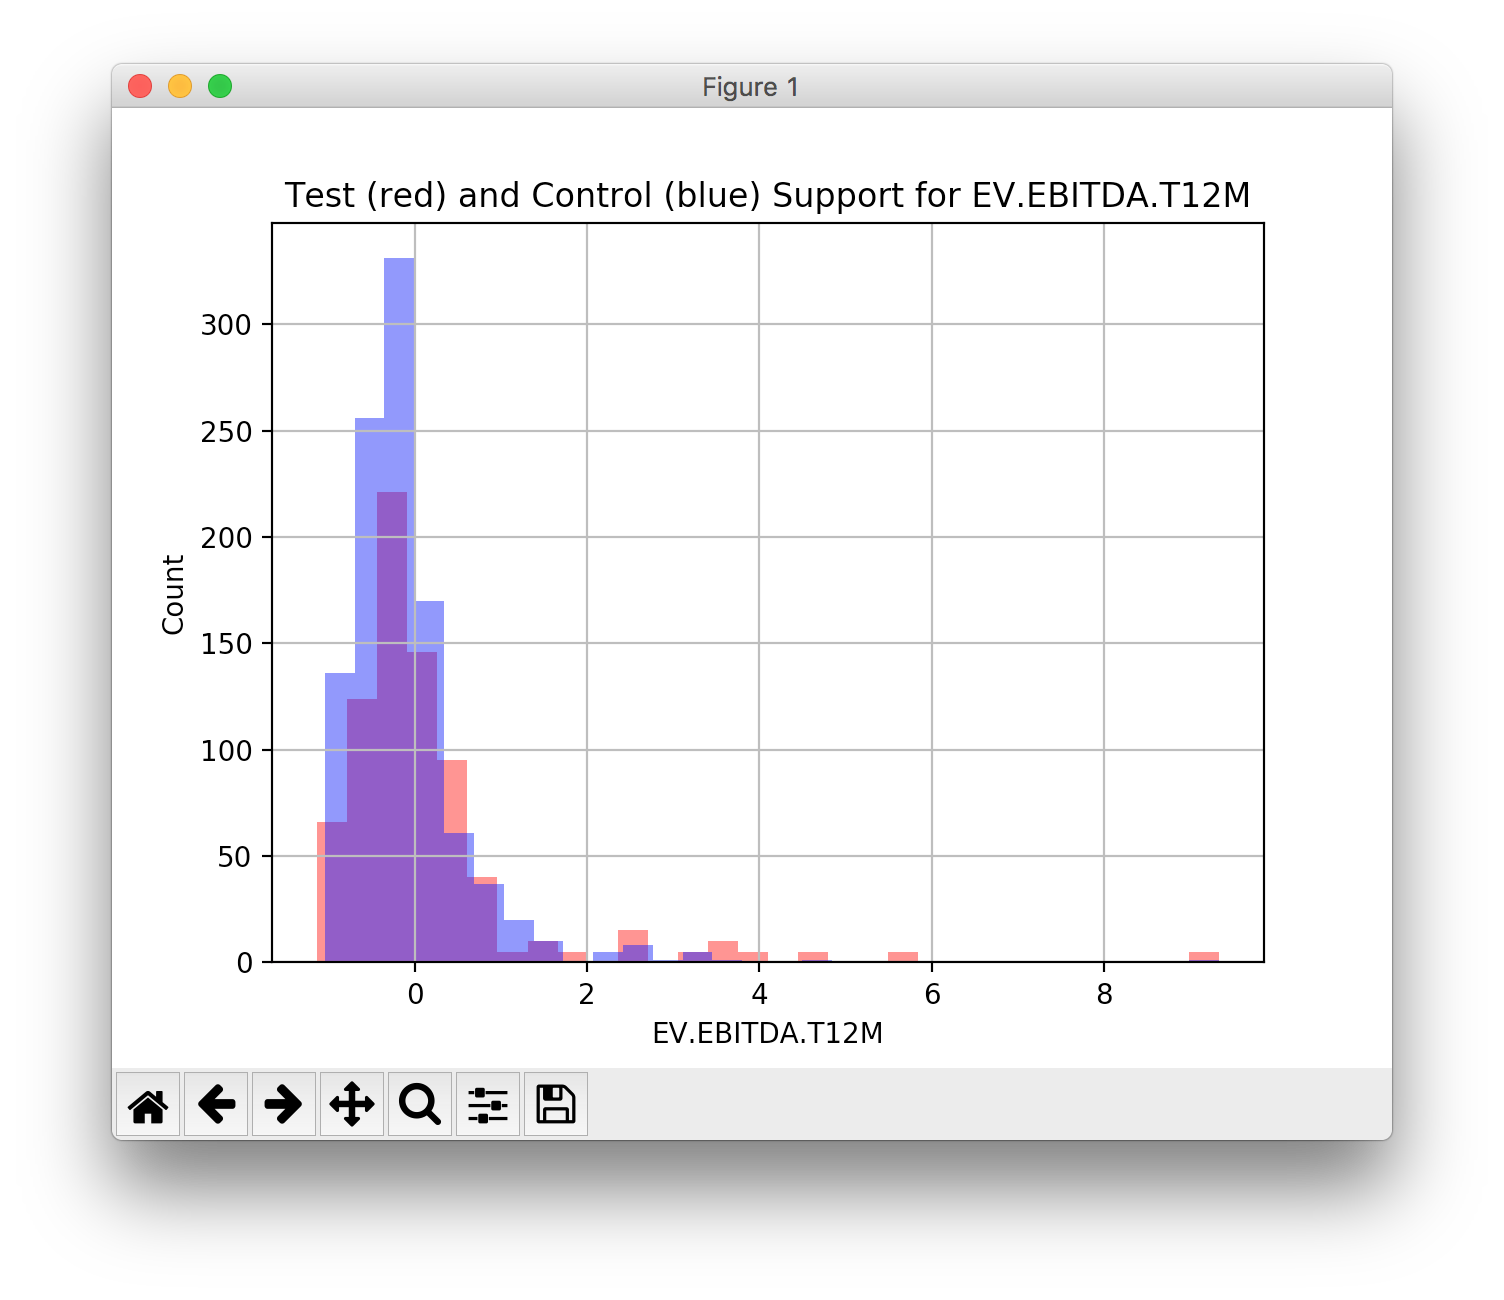
\includegraphics[width = 1.5in]{results/casual/BOD_Age_Rng/tobin/EV_EBITDA_T12M.png}} &
\subfigure[caption]{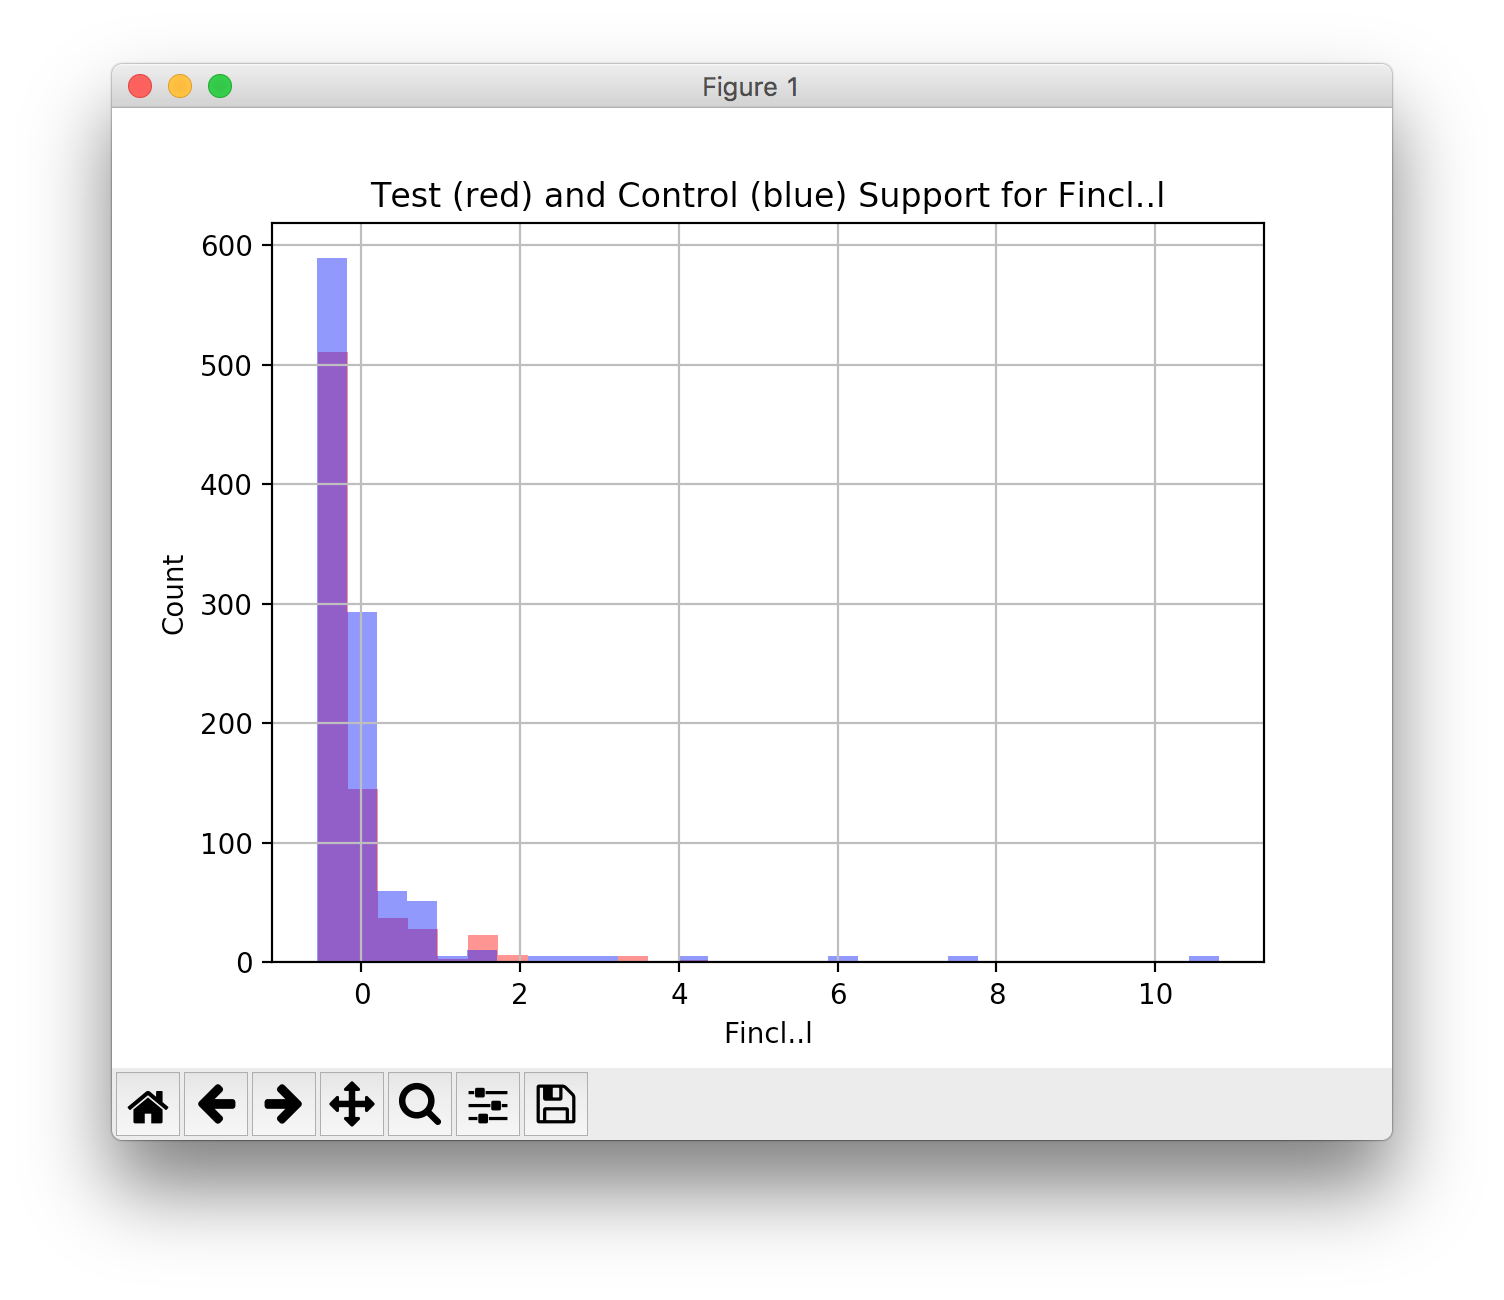
\includegraphics[width = 1.5in]{results/casual/BOD_Age_Rng/tobin/Fincl.png}} \\
\subfigure[caption]{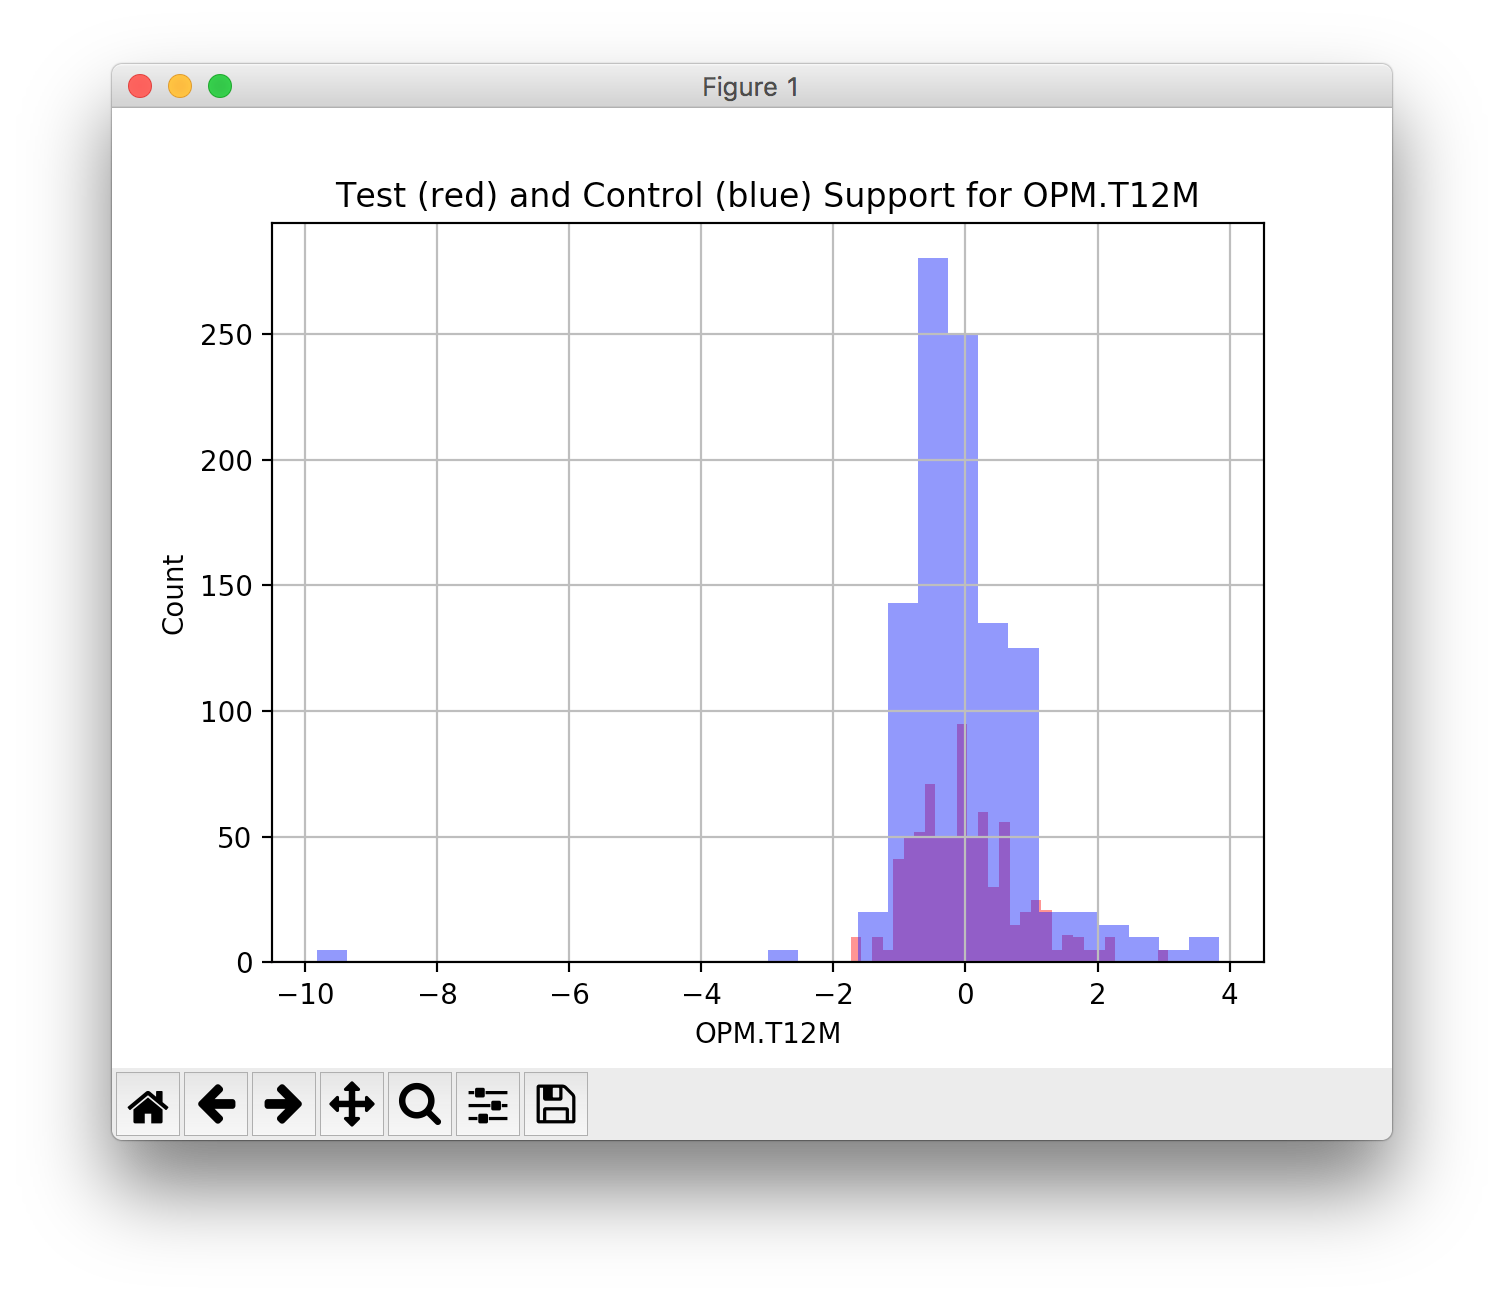
\includegraphics[width = 1.5in]{results/casual/BOD_Age_Rng/tobin/OPM_T12M.png}} &
\subfigure[caption]{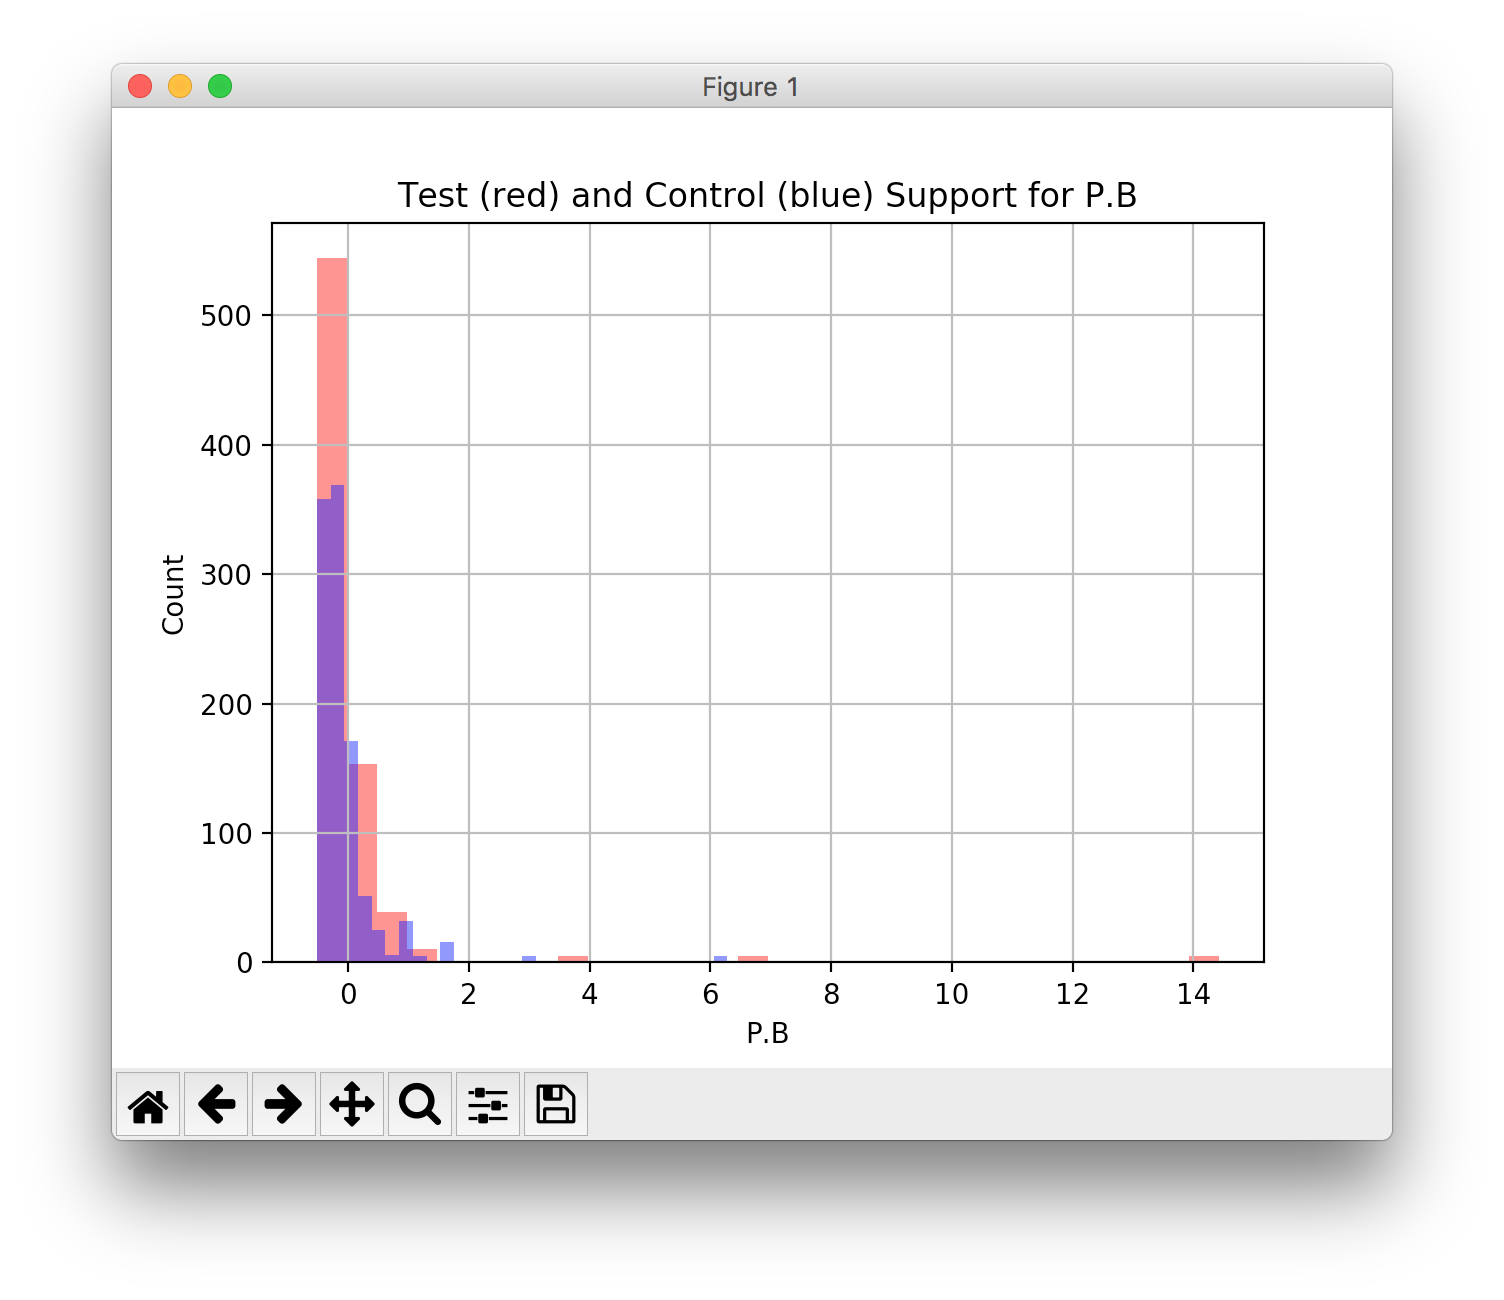
\includegraphics[width = 1.5in]{results/casual/BOD_Age_Rng/tobin/P_B.png}} &
\subfigure[caption]{\includegraphics[width = 1.5in]{results/casual/BOD_Age_Rng/tobin/P_EBITDA.png}} \\
\subfigure[caption]{\includegraphics[width = 1.5in]{results/casual/BOD_Age_Rng/tobin/ROC.png}} 
\end{tabular}
\caption{BOD.Age.Rng / SPX / Tobins Q}
\end{figure}
{\bf Interval: } {(0.028979256927540886, 0.054346807374190884, 0.079613783260607876) }
\clearpage


\begin{figure}[h!]
\begin{tabular}{ccc}
\subfigure[caption]{\includegraphics[width = 1.5in]{results/casual/BOD_Age_Rng/altman/Asset.png}} &
\subfigure[caption]{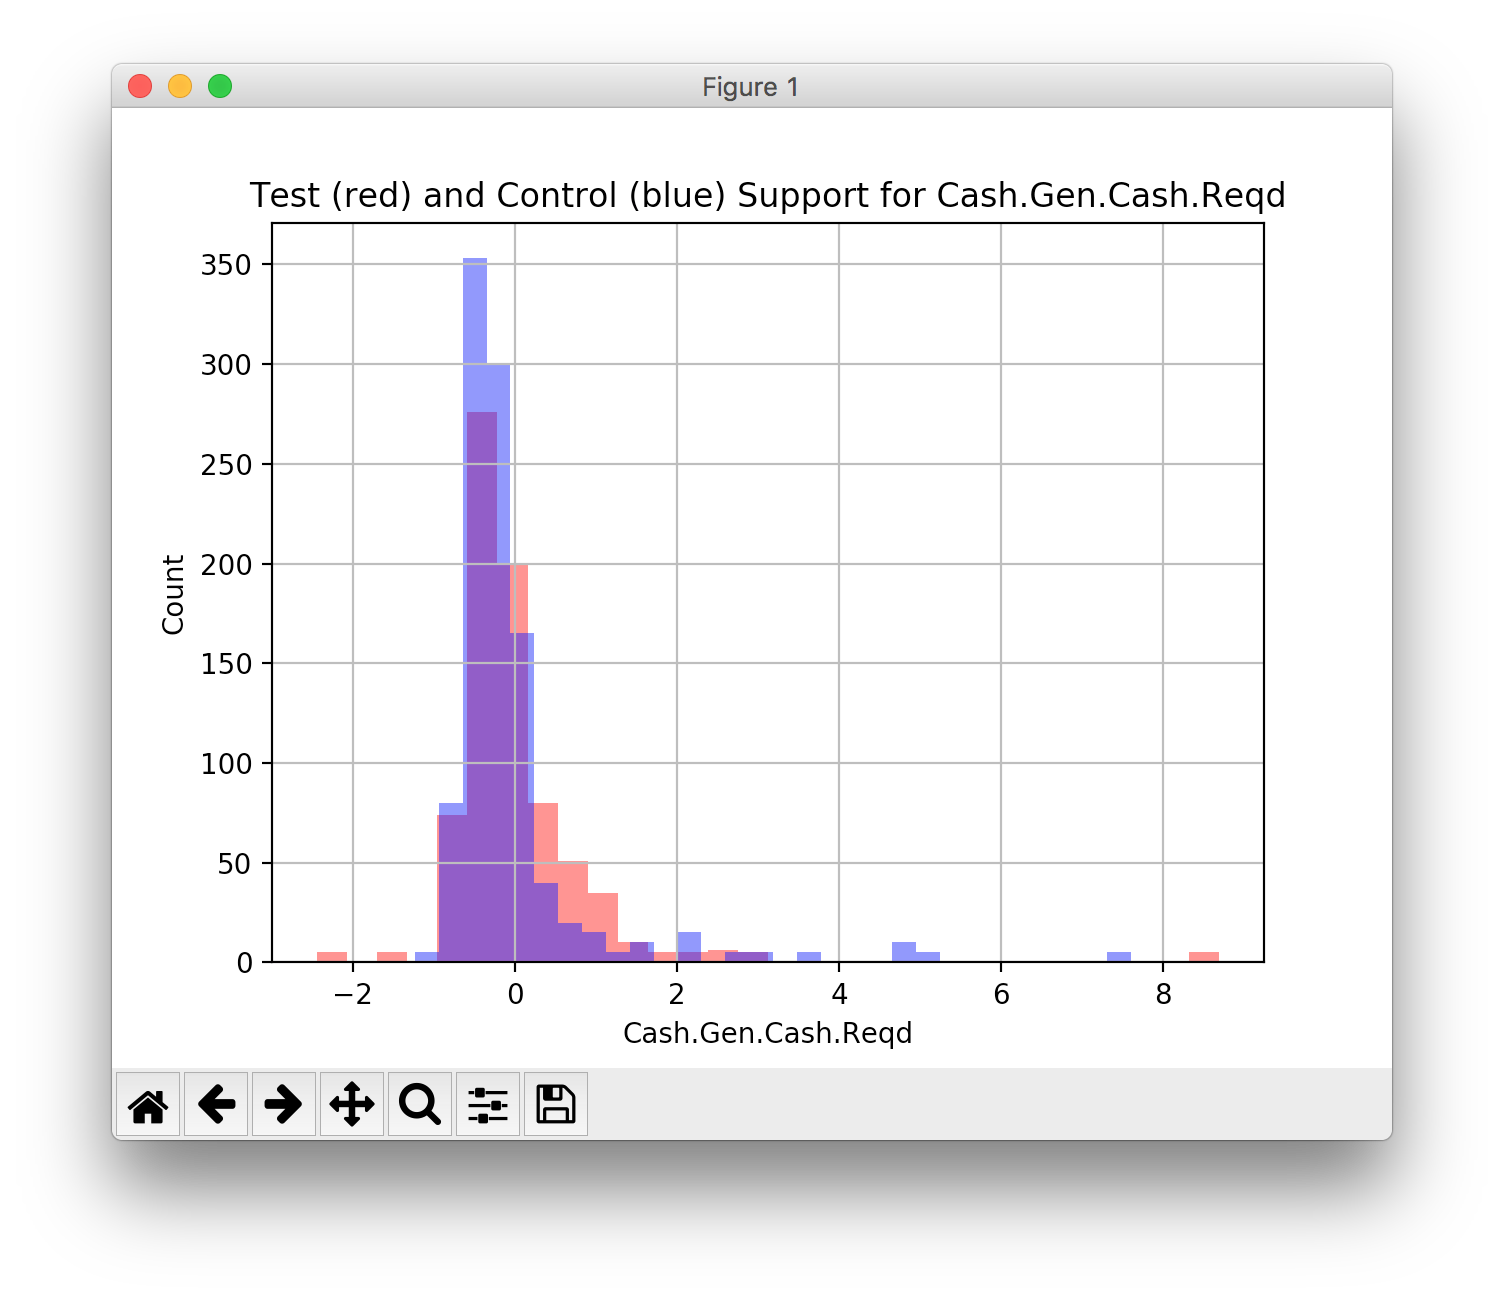
\includegraphics[width = 1.5in]{results/casual/BOD_Age_Rng/altman/Cash_Gen_Cash_Reqd.png}} &
\subfigure[caption]{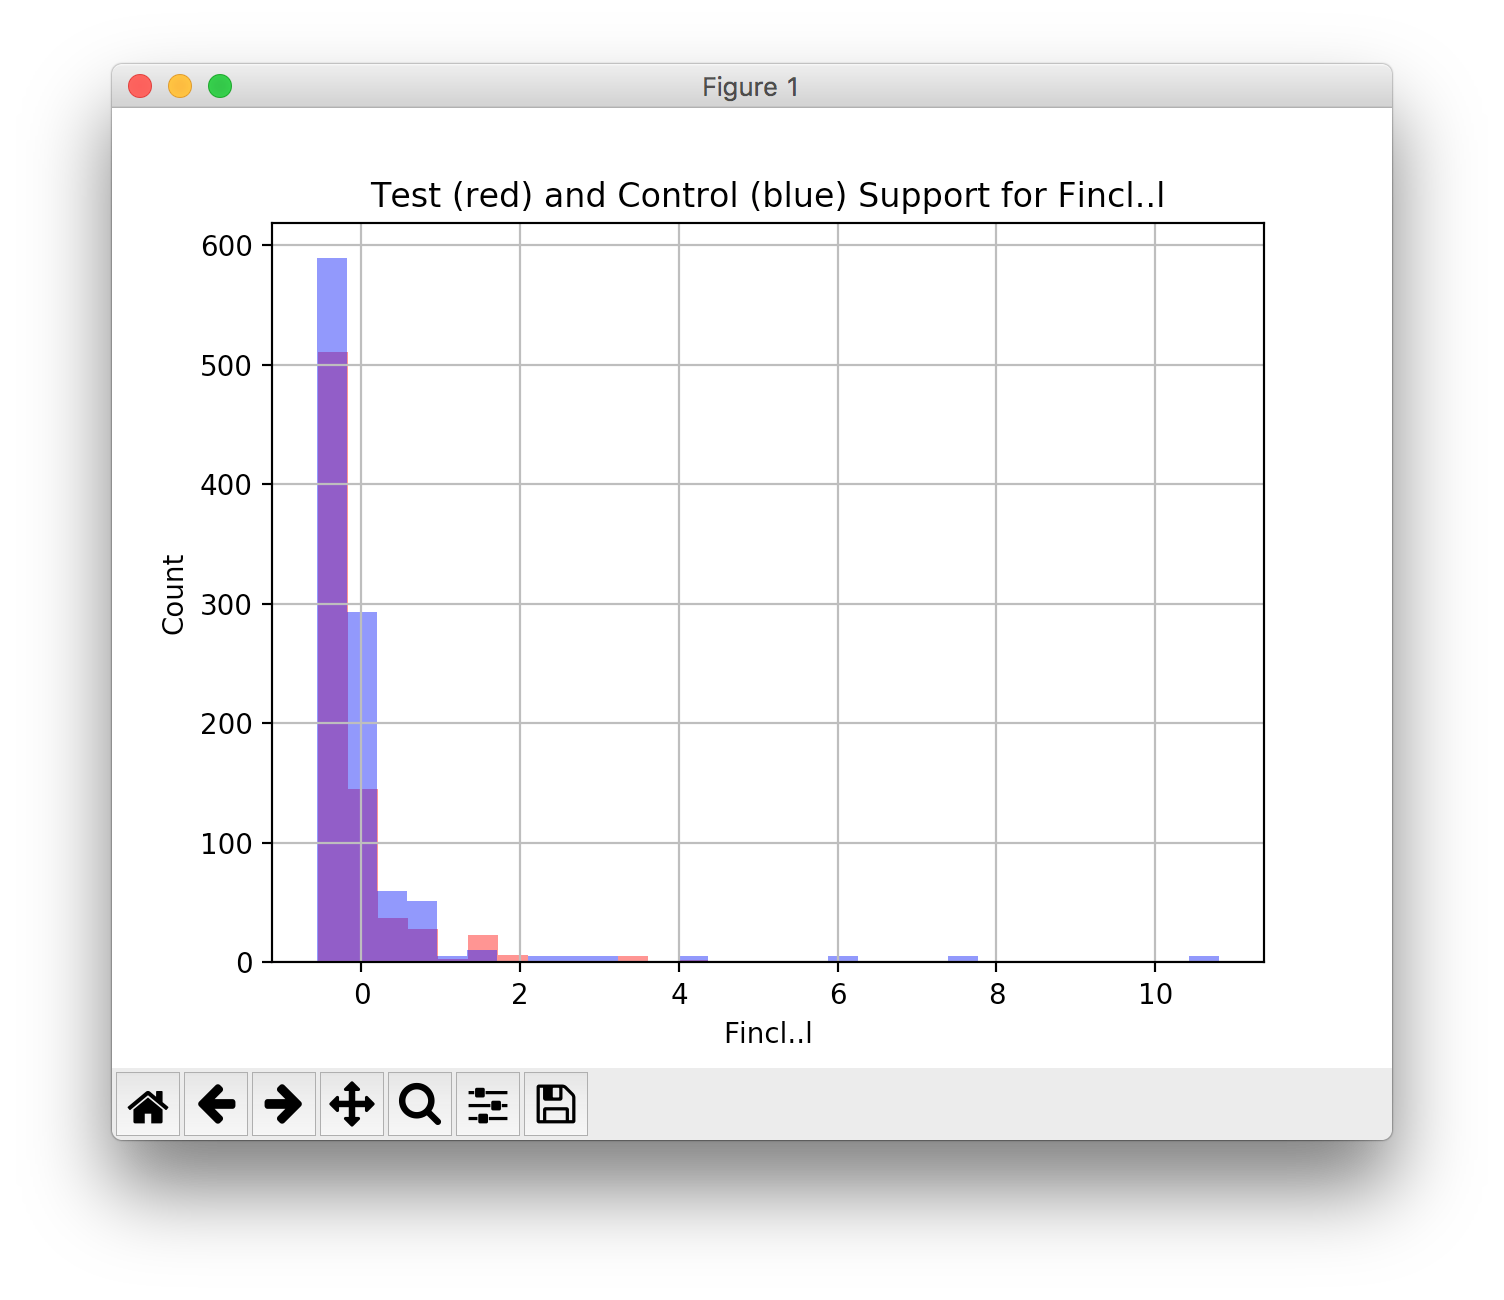
\includegraphics[width = 1.5in]{results/casual/BOD_Age_Rng/altman/Finc.png}} \\
\subfigure[caption]{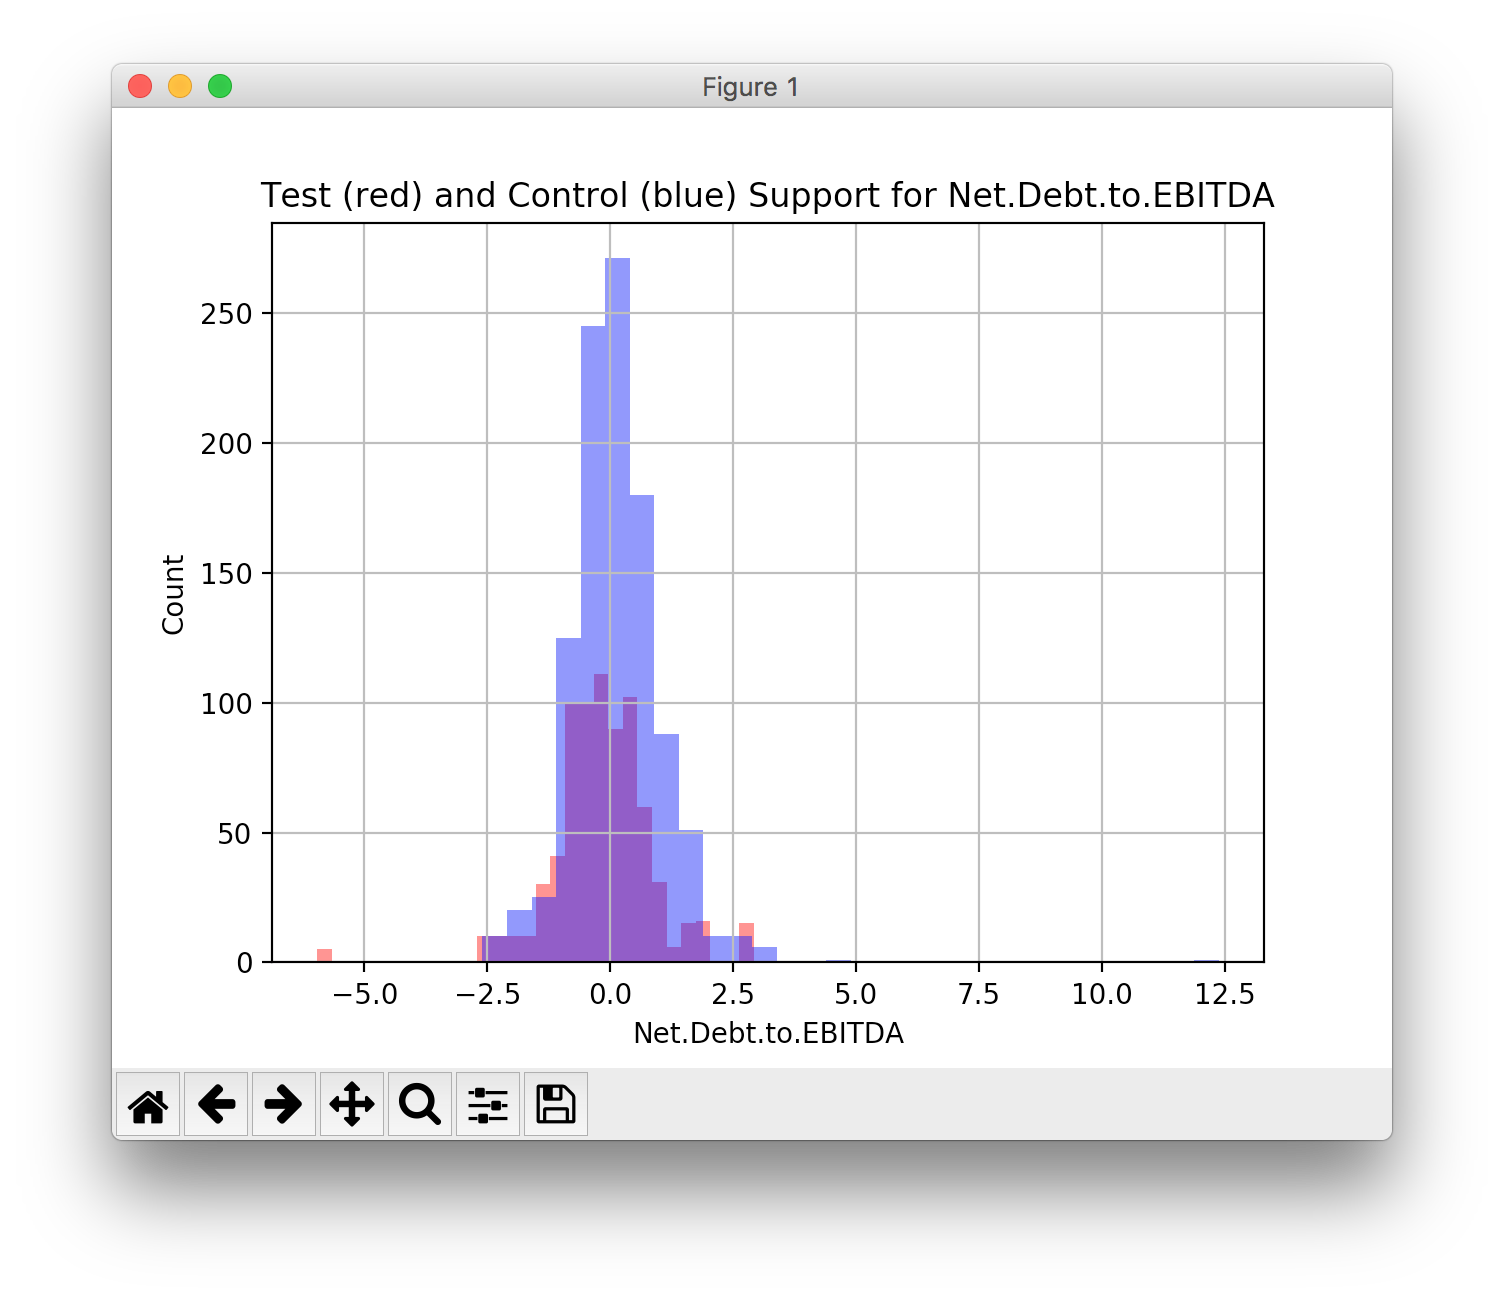
\includegraphics[width = 1.5in]{results/casual/BOD_Age_Rng/altman/Net_Debt_to_EBITDA.png}}&
\subfigure[caption]{\includegraphics[width = 1.5in]{results/casual/BOD_Age_Rng/altman/P_EBITDA.png}} &
\subfigure[caption]{\includegraphics[width = 1.5in]{results/casual/BOD_Age_Rng/altman/ROC.png}} \\
\subfigure[caption]{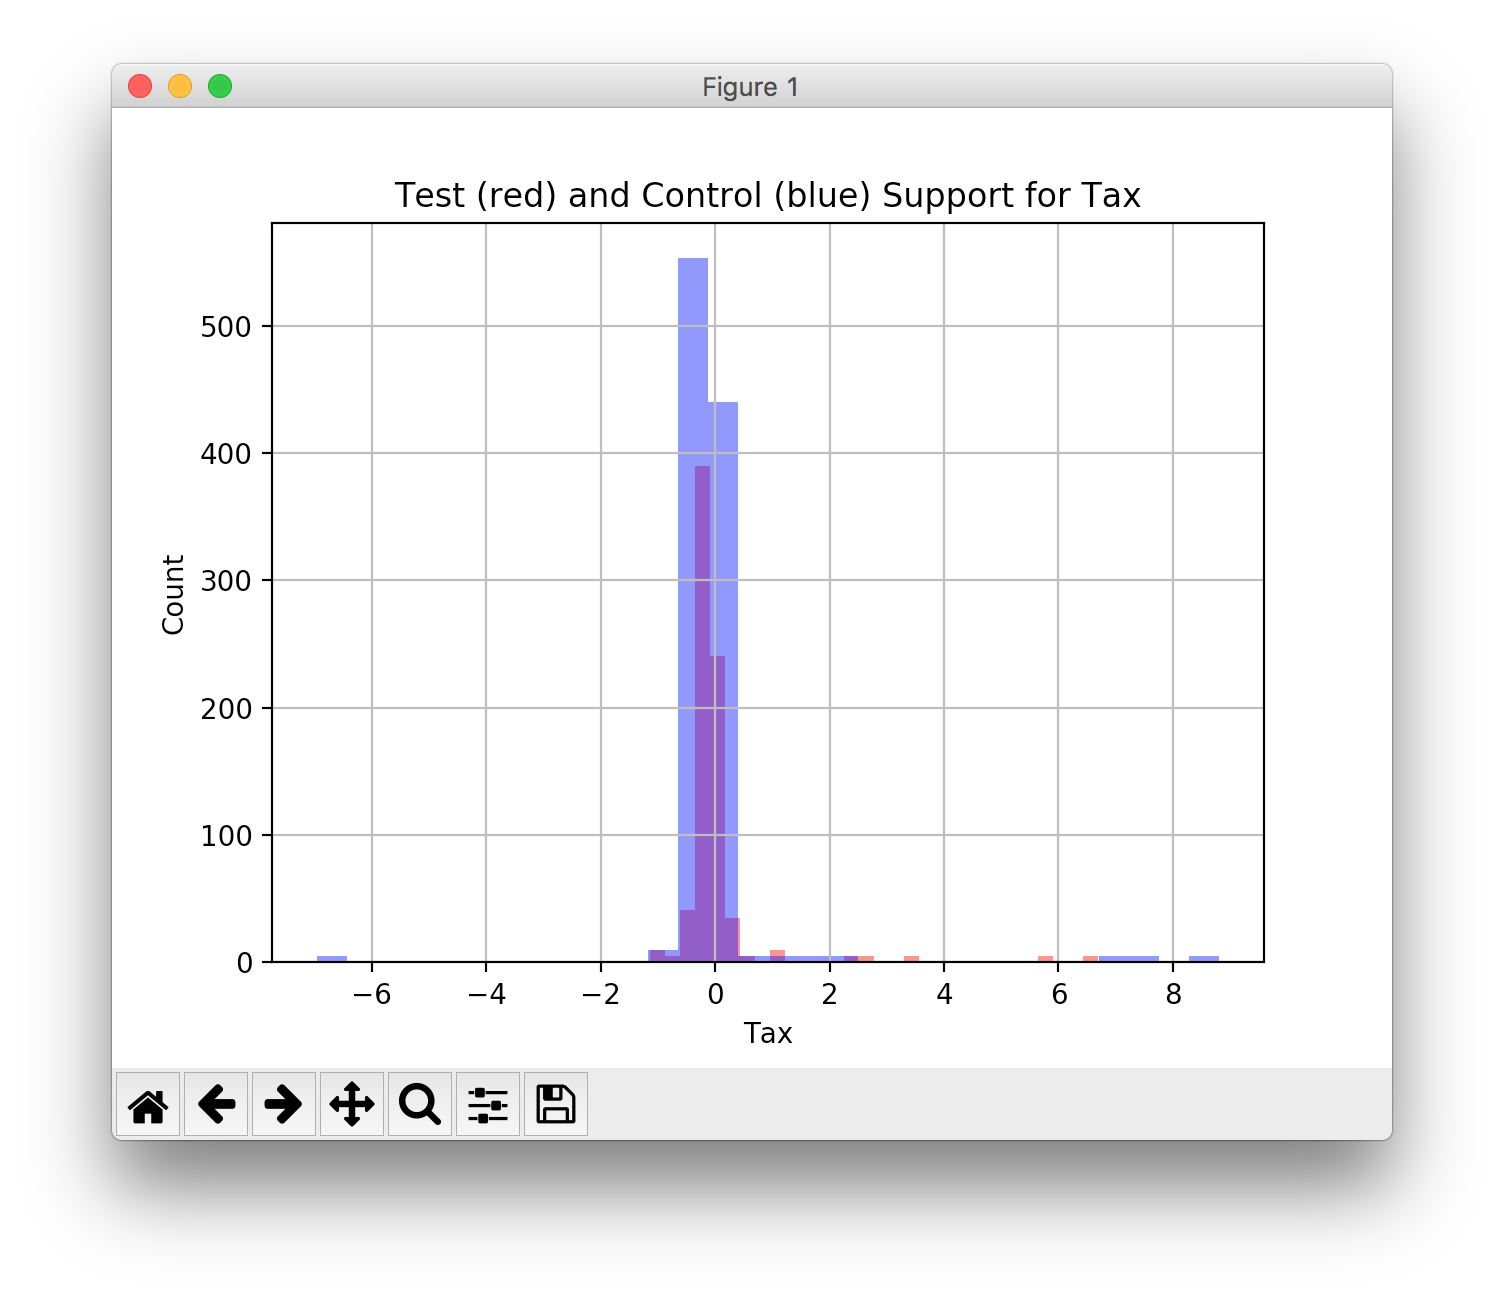
\includegraphics[width = 1.5in]{results/casual/BOD_Age_Rng/altman/Tax.png}} 
\end{tabular}
\caption{BOD.Age.Rng / Altman Z}
\end{figure}
{\bf Interval: } {(-0.009396477985696941, 0.012910009798425024, 0.037424725502139398)}
\clearpage



\clearpage

\subsection{Indep.Chrprsn.Feml.CEO.or.Equiv - SXXP}
\begin{figure}[h!]
\begin{tabular}{ccc}
\subfigure[caption]{\includegraphics[width = 1.5in]{results/casual/Indep_Chrprsn_Feml_CEO_or_Equiv/tobin/Asset.png}} &
\subfigure[caption]{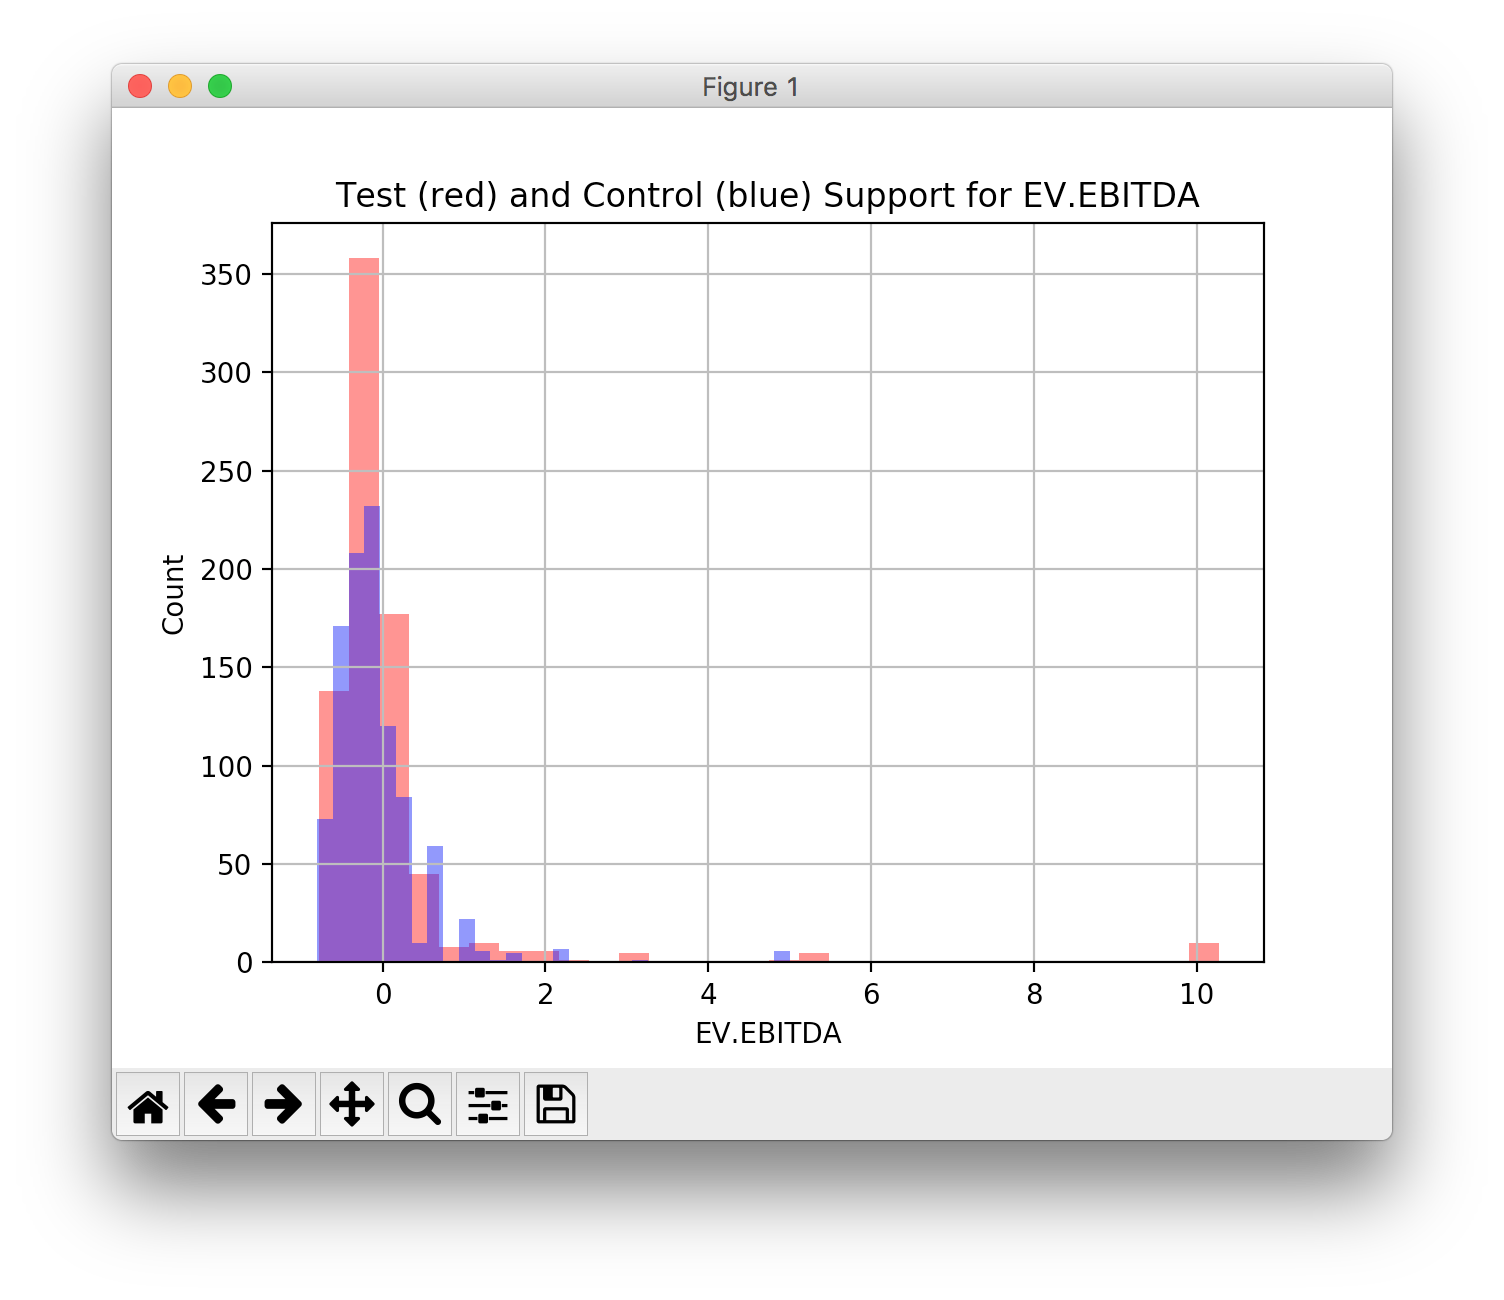
\includegraphics[width = 1.5in]{results/casual/Indep_Chrprsn_Feml_CEO_or_Equiv/tobin/EV_EBITDA.png}} &
\subfigure[caption]{\includegraphics[width = 1.5in]{results/casual/Indep_Chrprsn_Feml_CEO_or_Equiv/tobin/Fincl.png}} \\
\subfigure[caption]{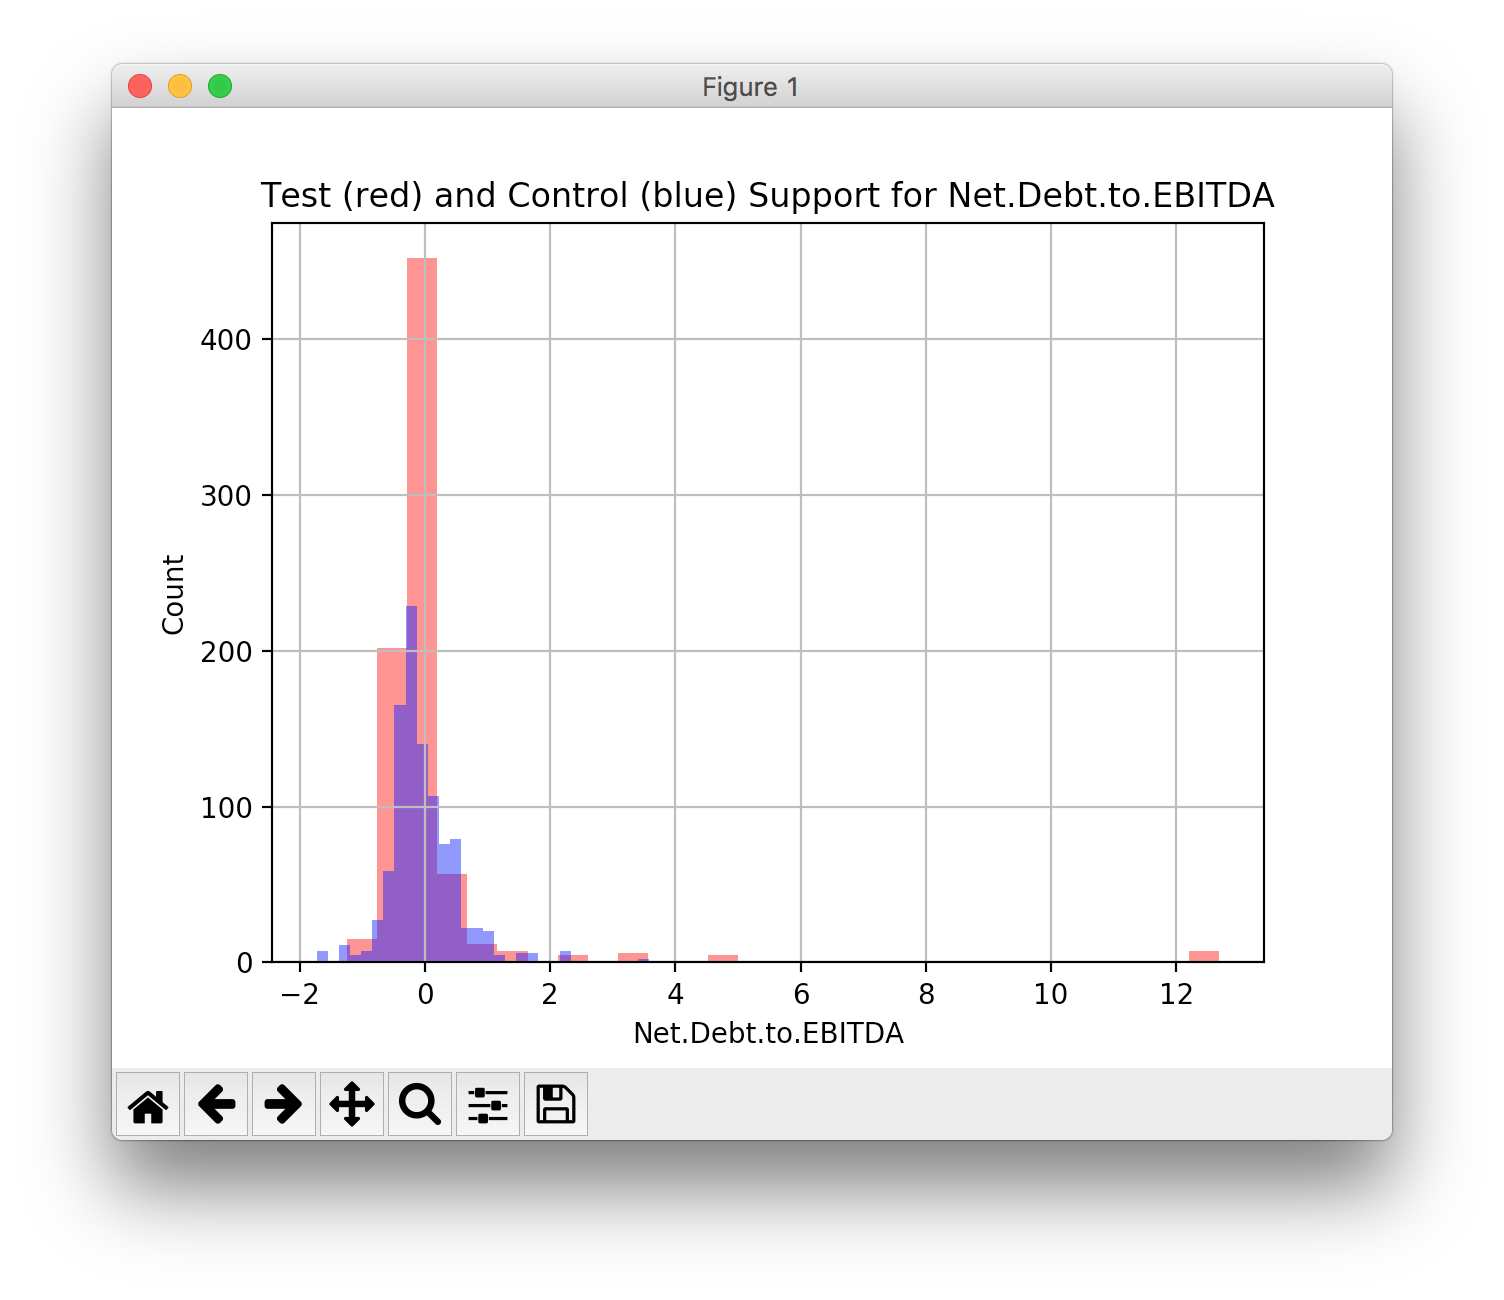
\includegraphics[width = 1.5in]{results/casual/Indep_Chrprsn_Feml_CEO_or_Equiv/tobin/Net_Debt_to_Ebitda.png}} &
\subfigure[caption]{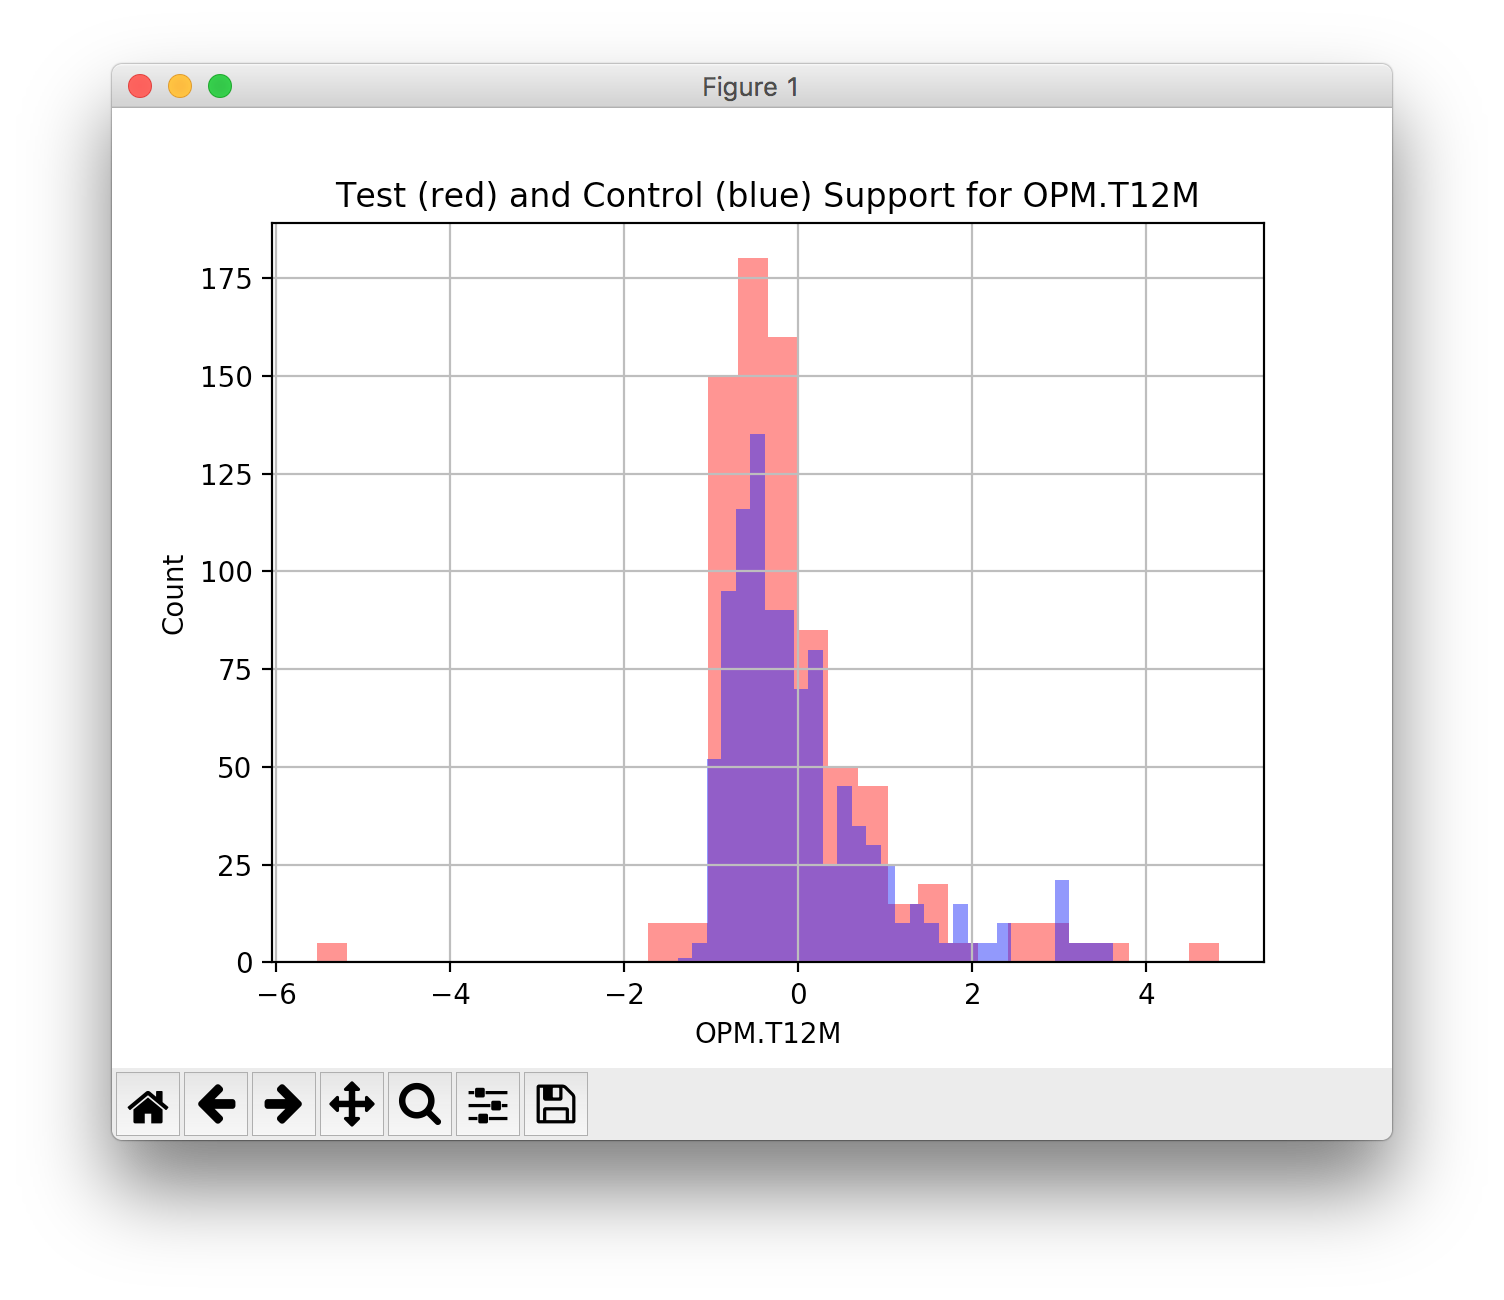
\includegraphics[width = 1.5in]{results/casual/Indep_Chrprsn_Feml_CEO_or_Equiv/tobin/OPM_T12M.png}} &
\subfigure[caption]{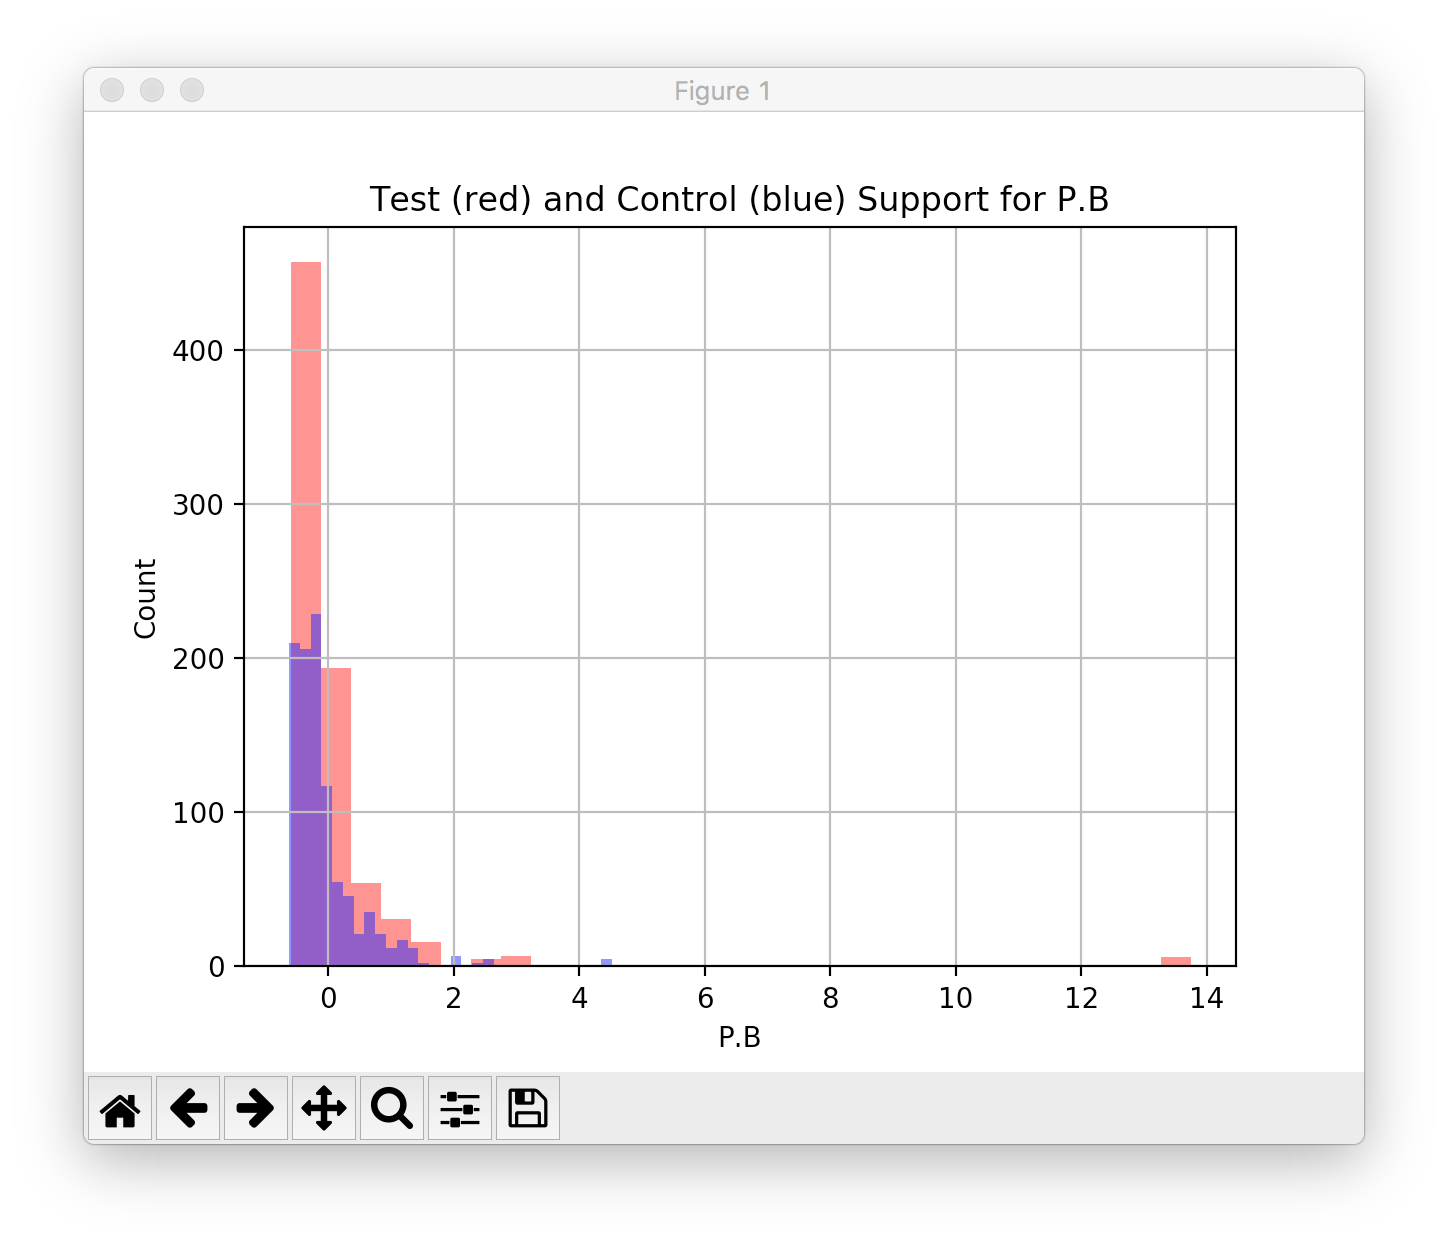
\includegraphics[width = 1.5in]{results/casual/Indep_Chrprsn_Feml_CEO_or_Equiv/tobin/PB.png}} \\
\subfigure[caption]{\includegraphics[width = 1.5in]{results/casual/Indep_Chrprsn_Feml_CEO_or_Equiv/tobin/PE.png}}  &
\subfigure[caption]{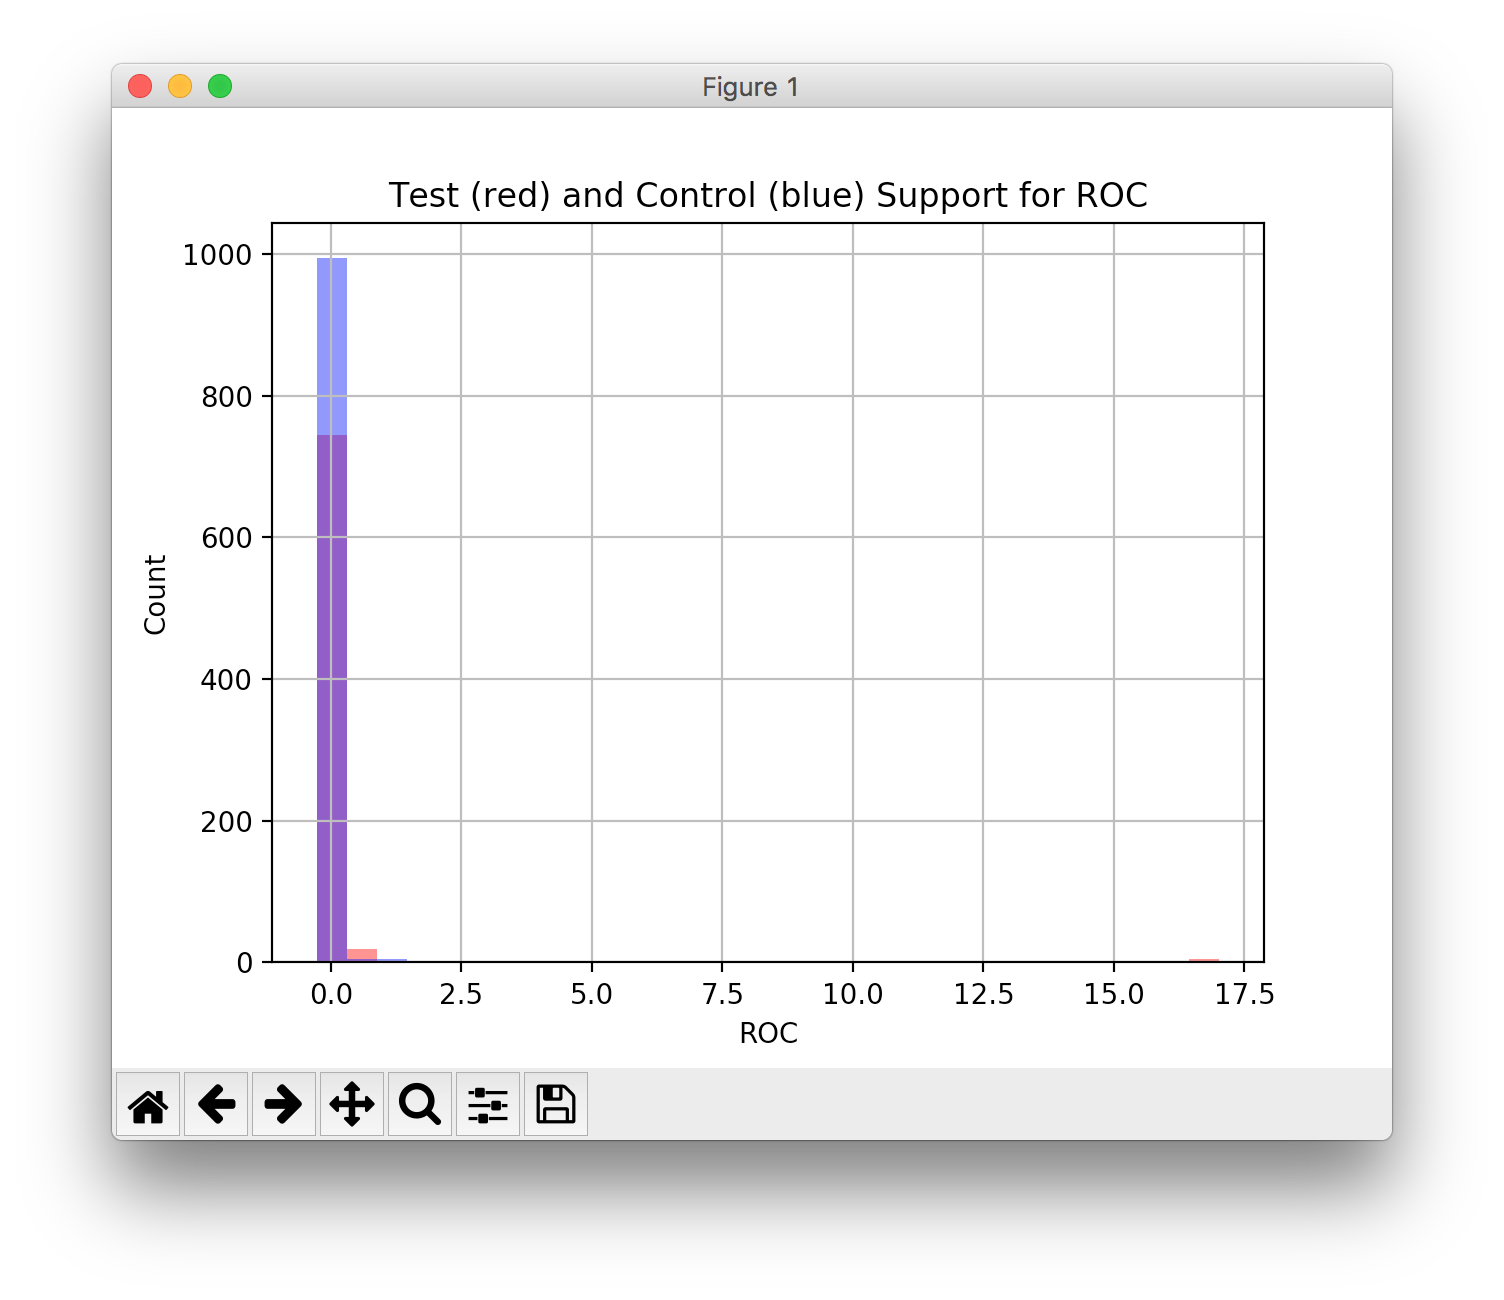
\includegraphics[width = 1.5in]{results/casual/Indep_Chrprsn_Feml_CEO_or_Equiv/tobin/ROC.png}}  &
\subfigure[caption]{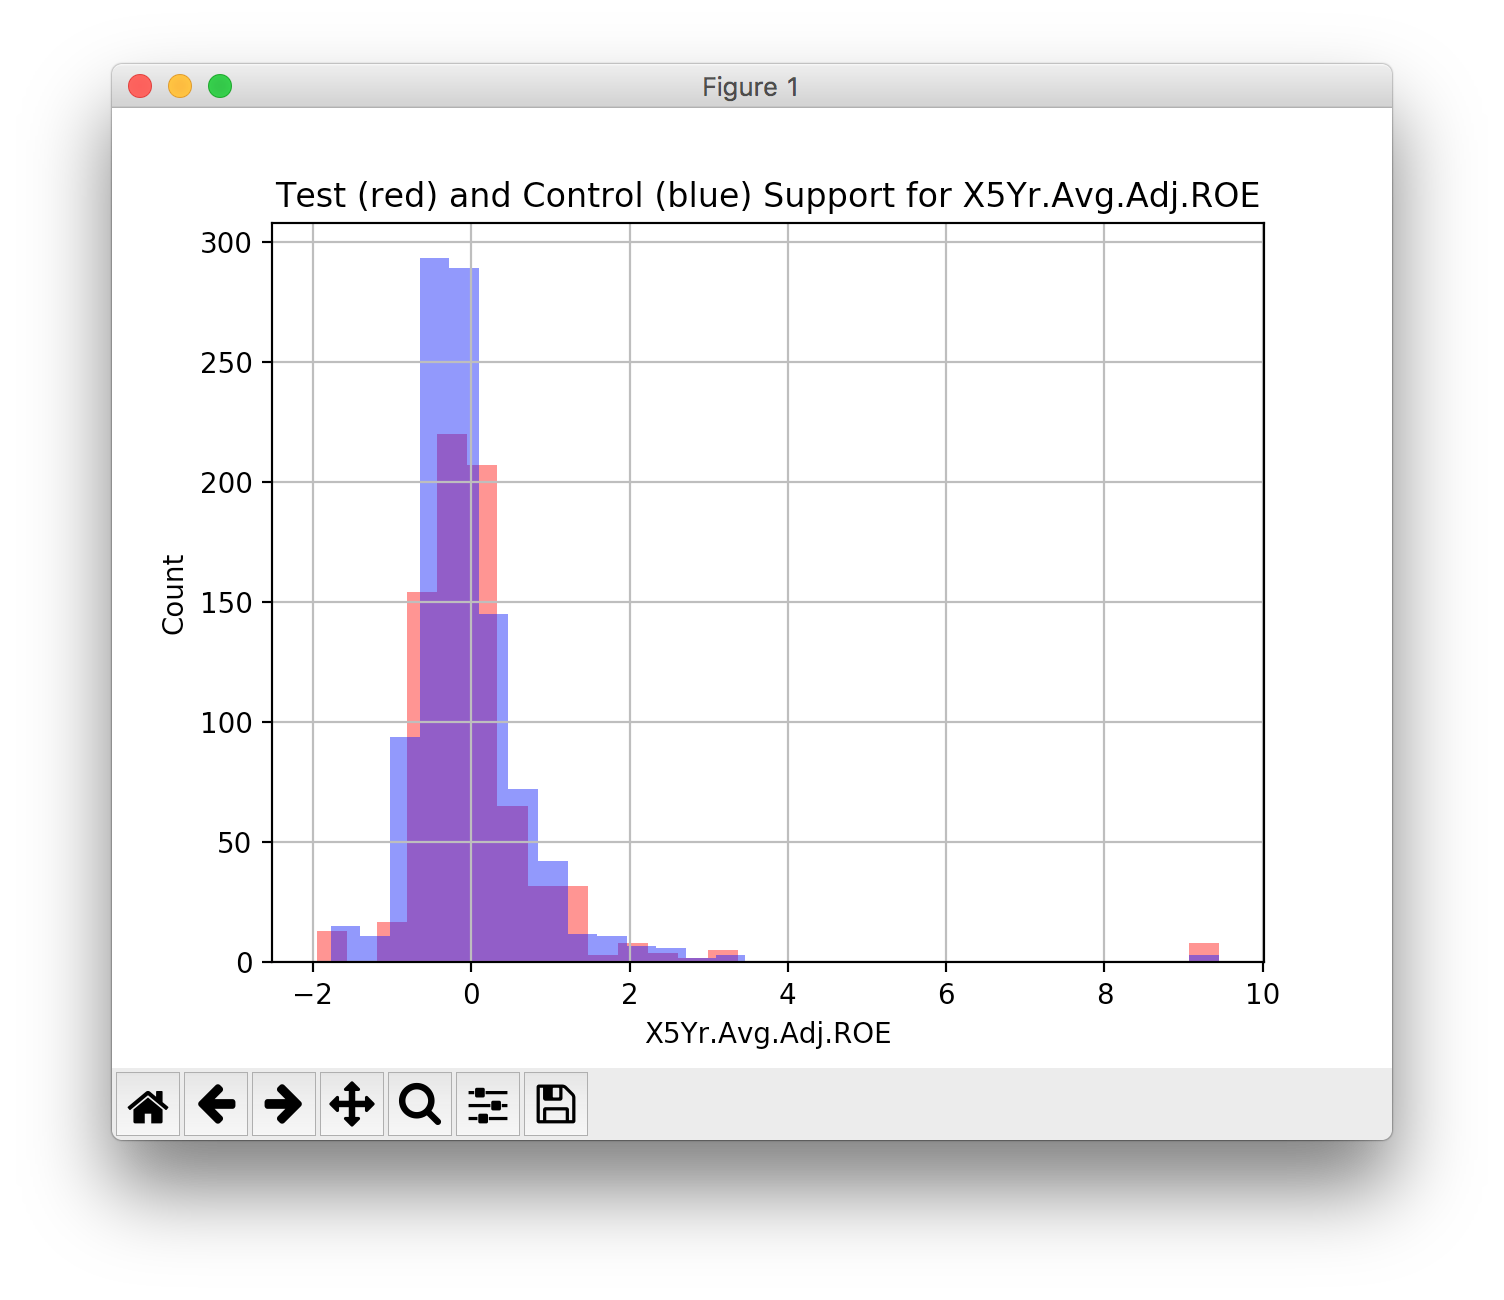
\includegraphics[width = 1.5in]{results/casual/Indep_Chrprsn_Feml_CEO_or_Equiv/tobin/X5Yr_Avg_Adj_ROE.png}} 
\end{tabular}
\caption{Indep\_Chrprsn\_Feml\_CEO\_or\_Equiv / Tobins Q}
\end{figure}
{\bf Interval: } {(0.04875811045630455, 0.07241903781028242, 0.096285668424400075)}
\clearpage

\begin{figure}[h!]
\begin{tabular}{ccc}
\subfigure[caption]{\includegraphics[width = 1.5in]{results/casual/Indep_Chrprsn_Feml_CEO_or_Equiv/altman/Asset.png}} &
\subfigure[caption]{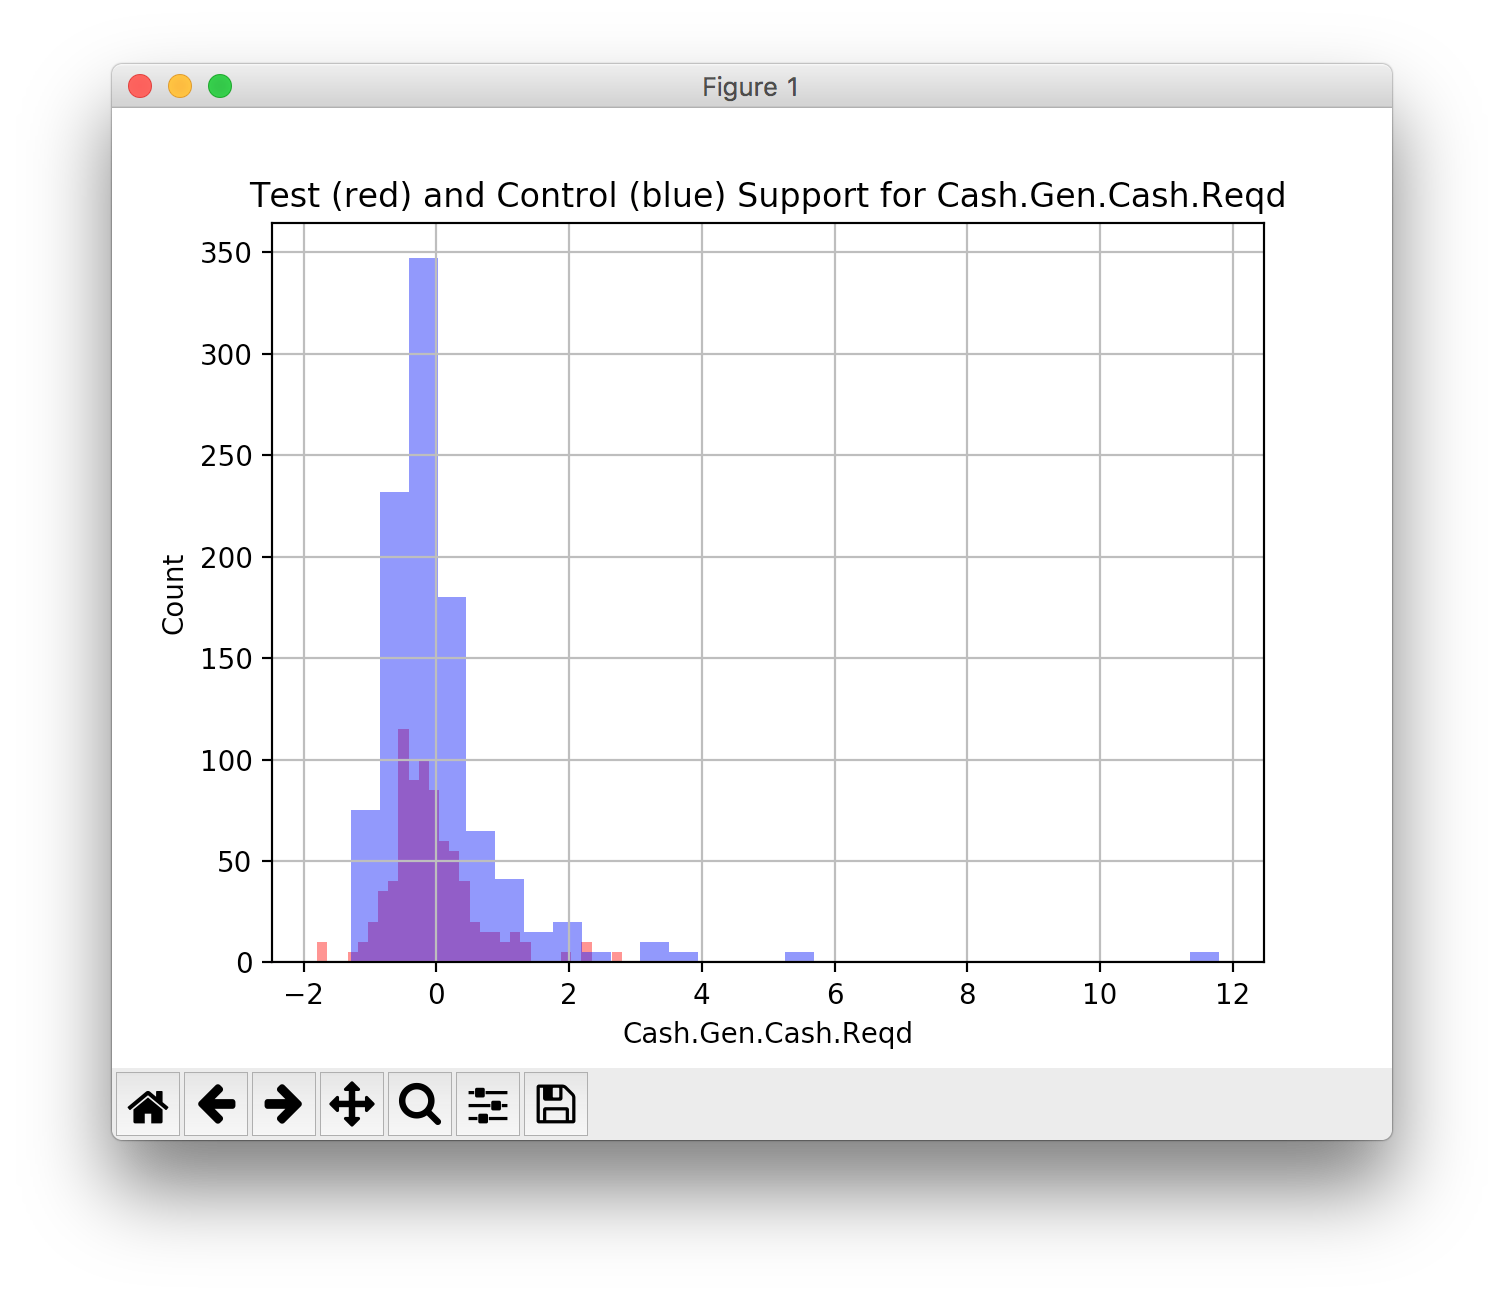
\includegraphics[width = 1.5in]{results/casual/Indep_Chrprsn_Feml_CEO_or_Equiv/altman/Cash_Gen_Cash_Reqd.png}} &
\subfigure[caption]{\includegraphics[width = 1.5in]{results/casual/Indep_Chrprsn_Feml_CEO_or_Equiv/altman/Fincl.png}} \\
\subfigure[caption]{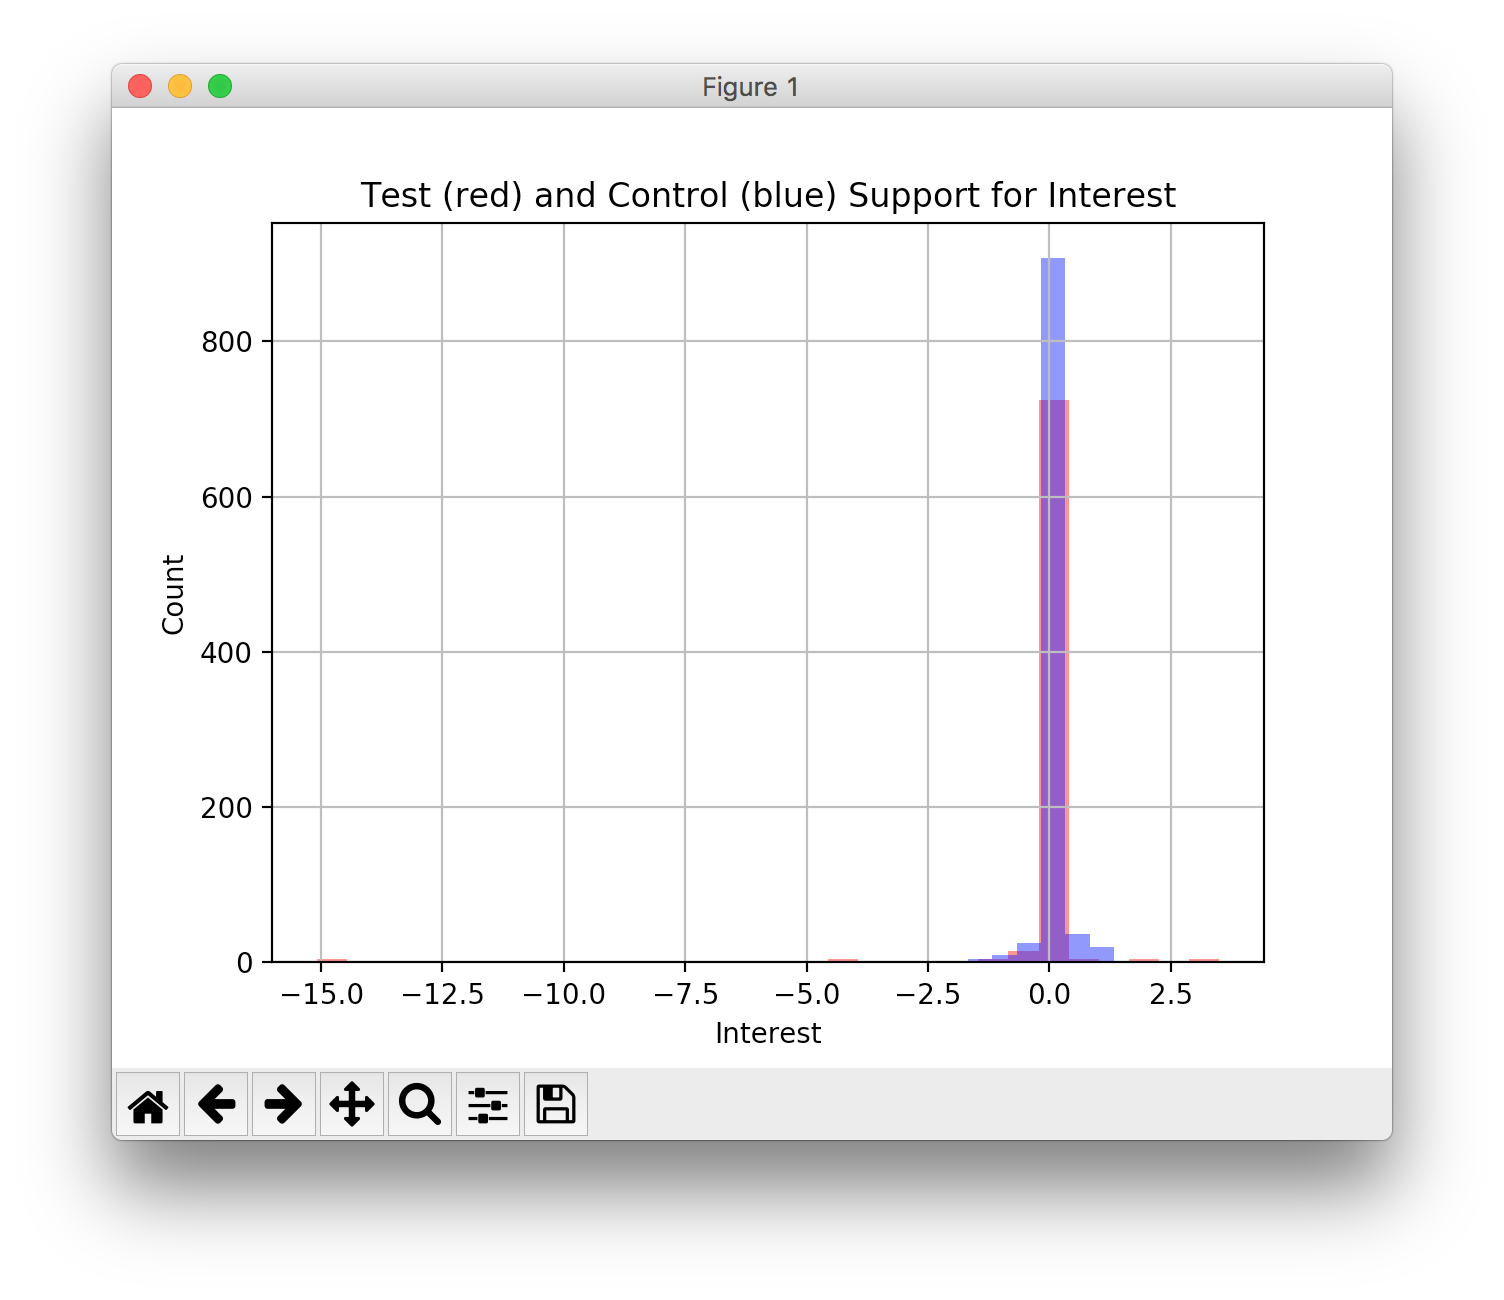
\includegraphics[width = 1.5in]{results/casual/Indep_Chrprsn_Feml_CEO_or_Equiv/altman/Interest.png}} &
\subfigure[caption]{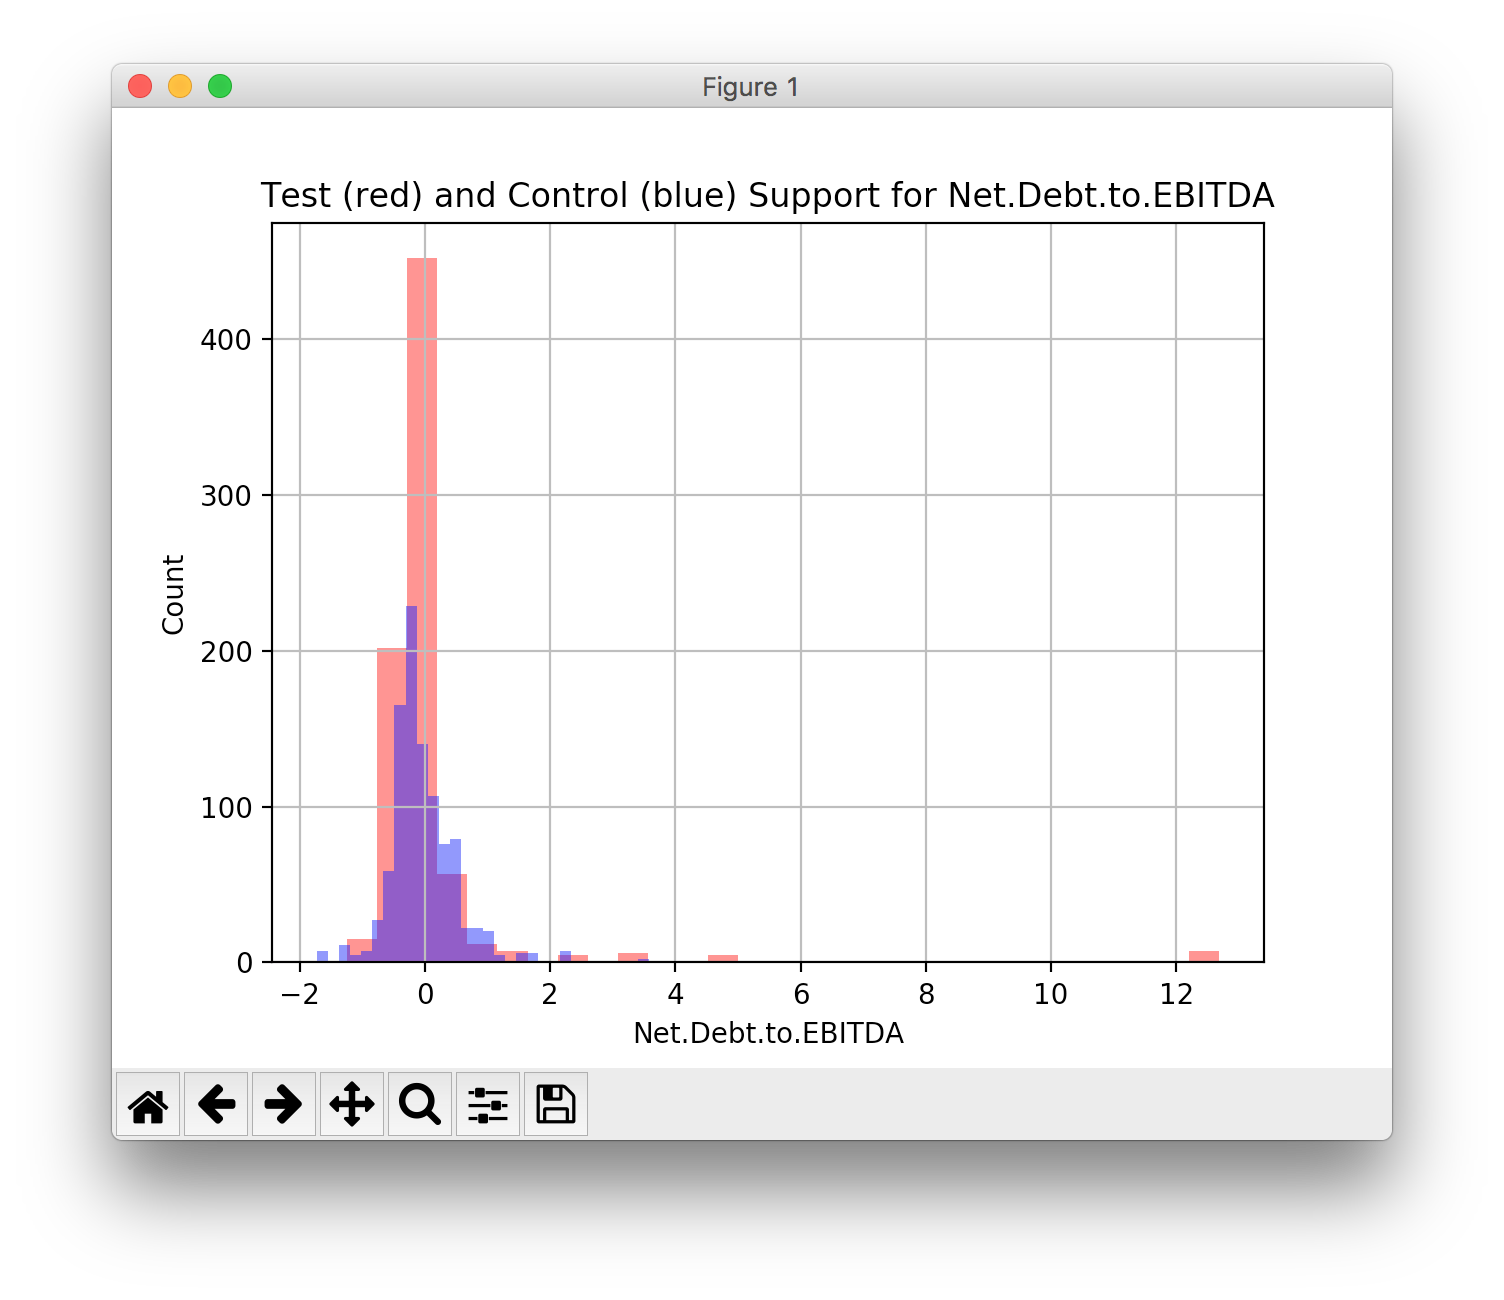
\includegraphics[width = 1.5in]{results/casual/Indep_Chrprsn_Feml_CEO_or_Equiv/altman/Net_Debt_to_EBITDA.png}} &
\subfigure[caption]{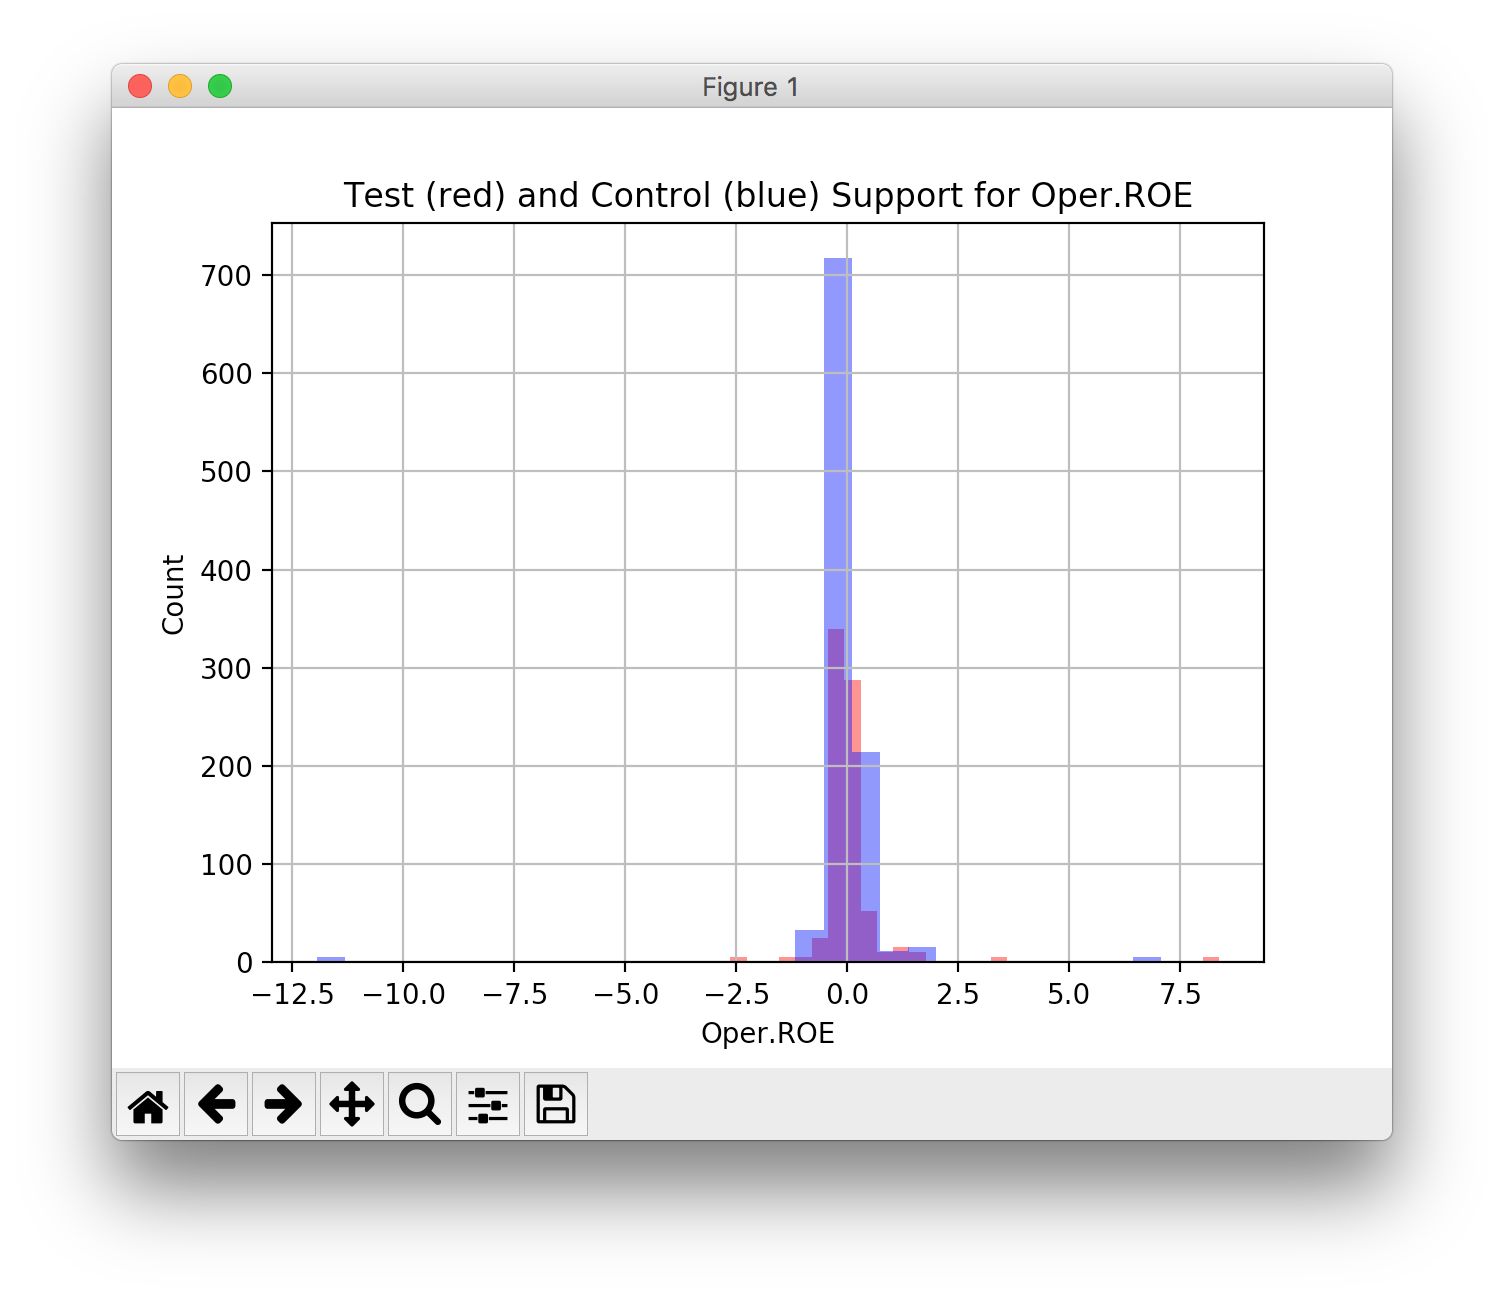
\includegraphics[width = 1.5in]{results/casual/Indep_Chrprsn_Feml_CEO_or_Equiv/altman/Oper_ROE.png}} \\
\subfigure[caption]{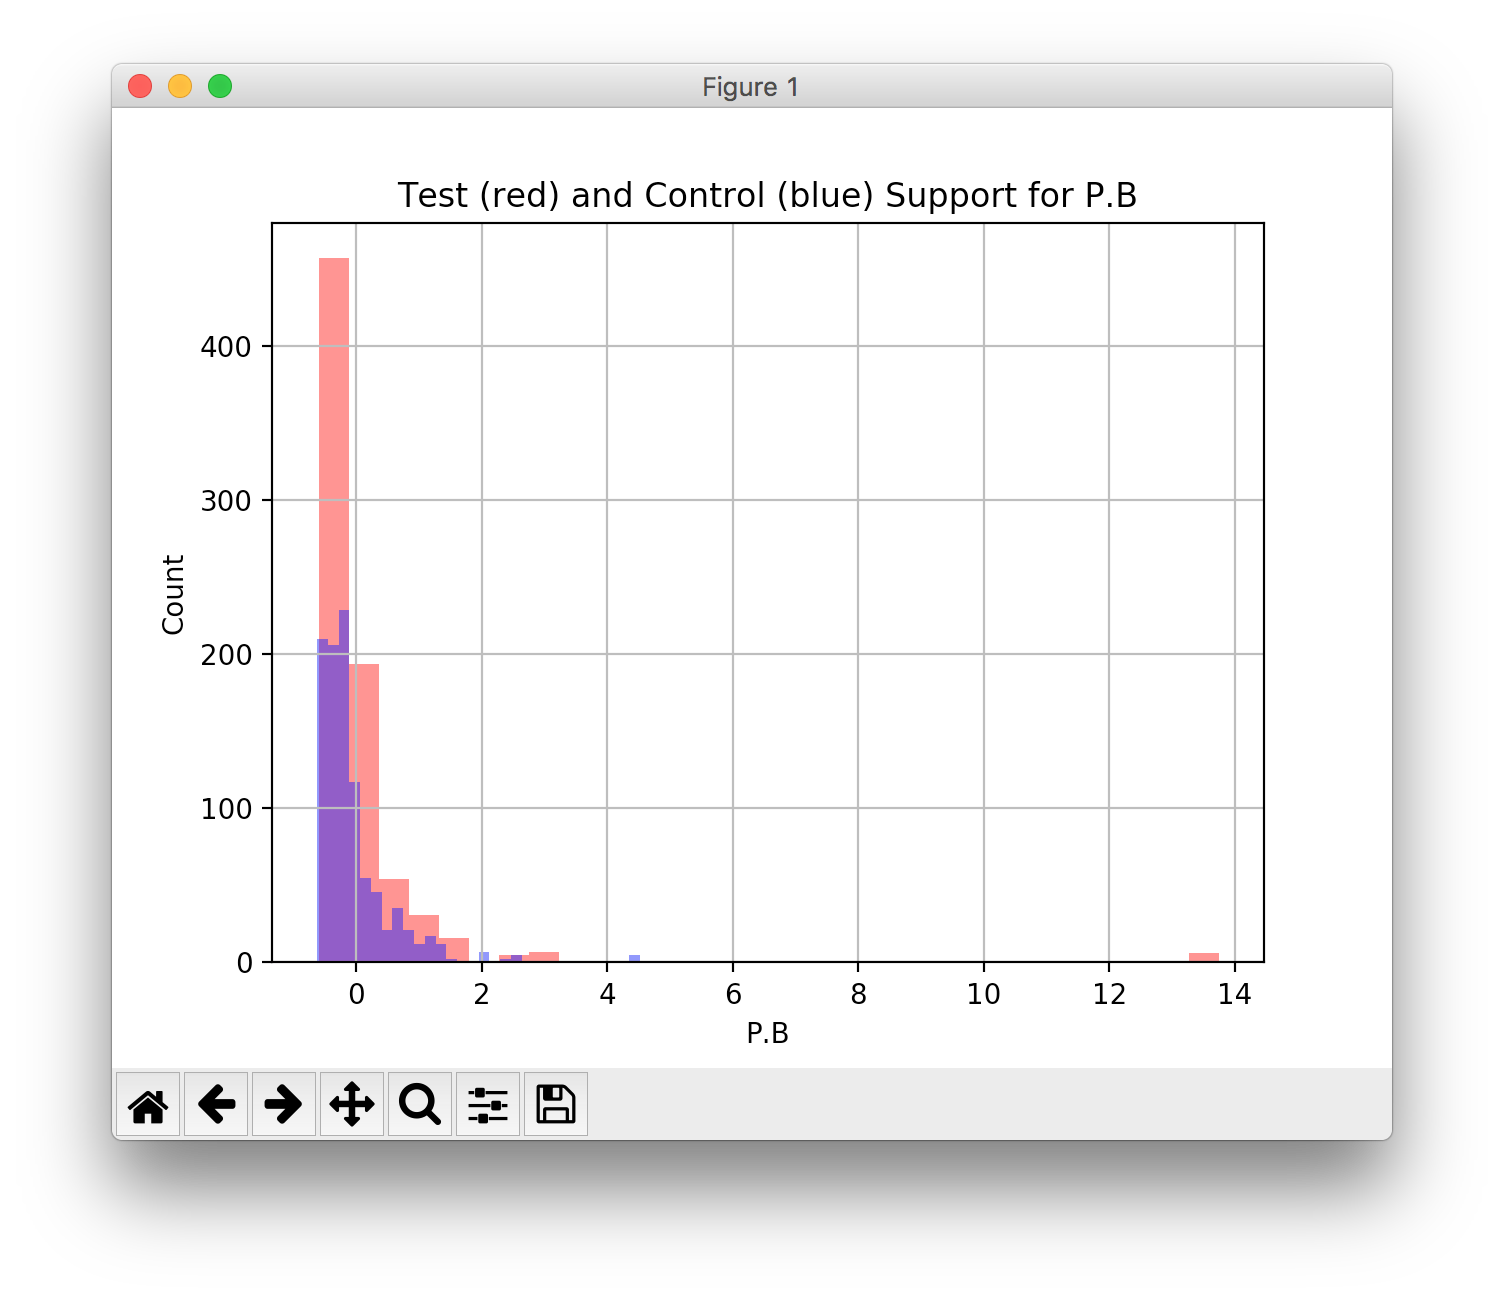
\includegraphics[width = 1.5in]{results/casual/Indep_Chrprsn_Feml_CEO_or_Equiv/altman/P_B.png}}  &
\subfigure[caption]{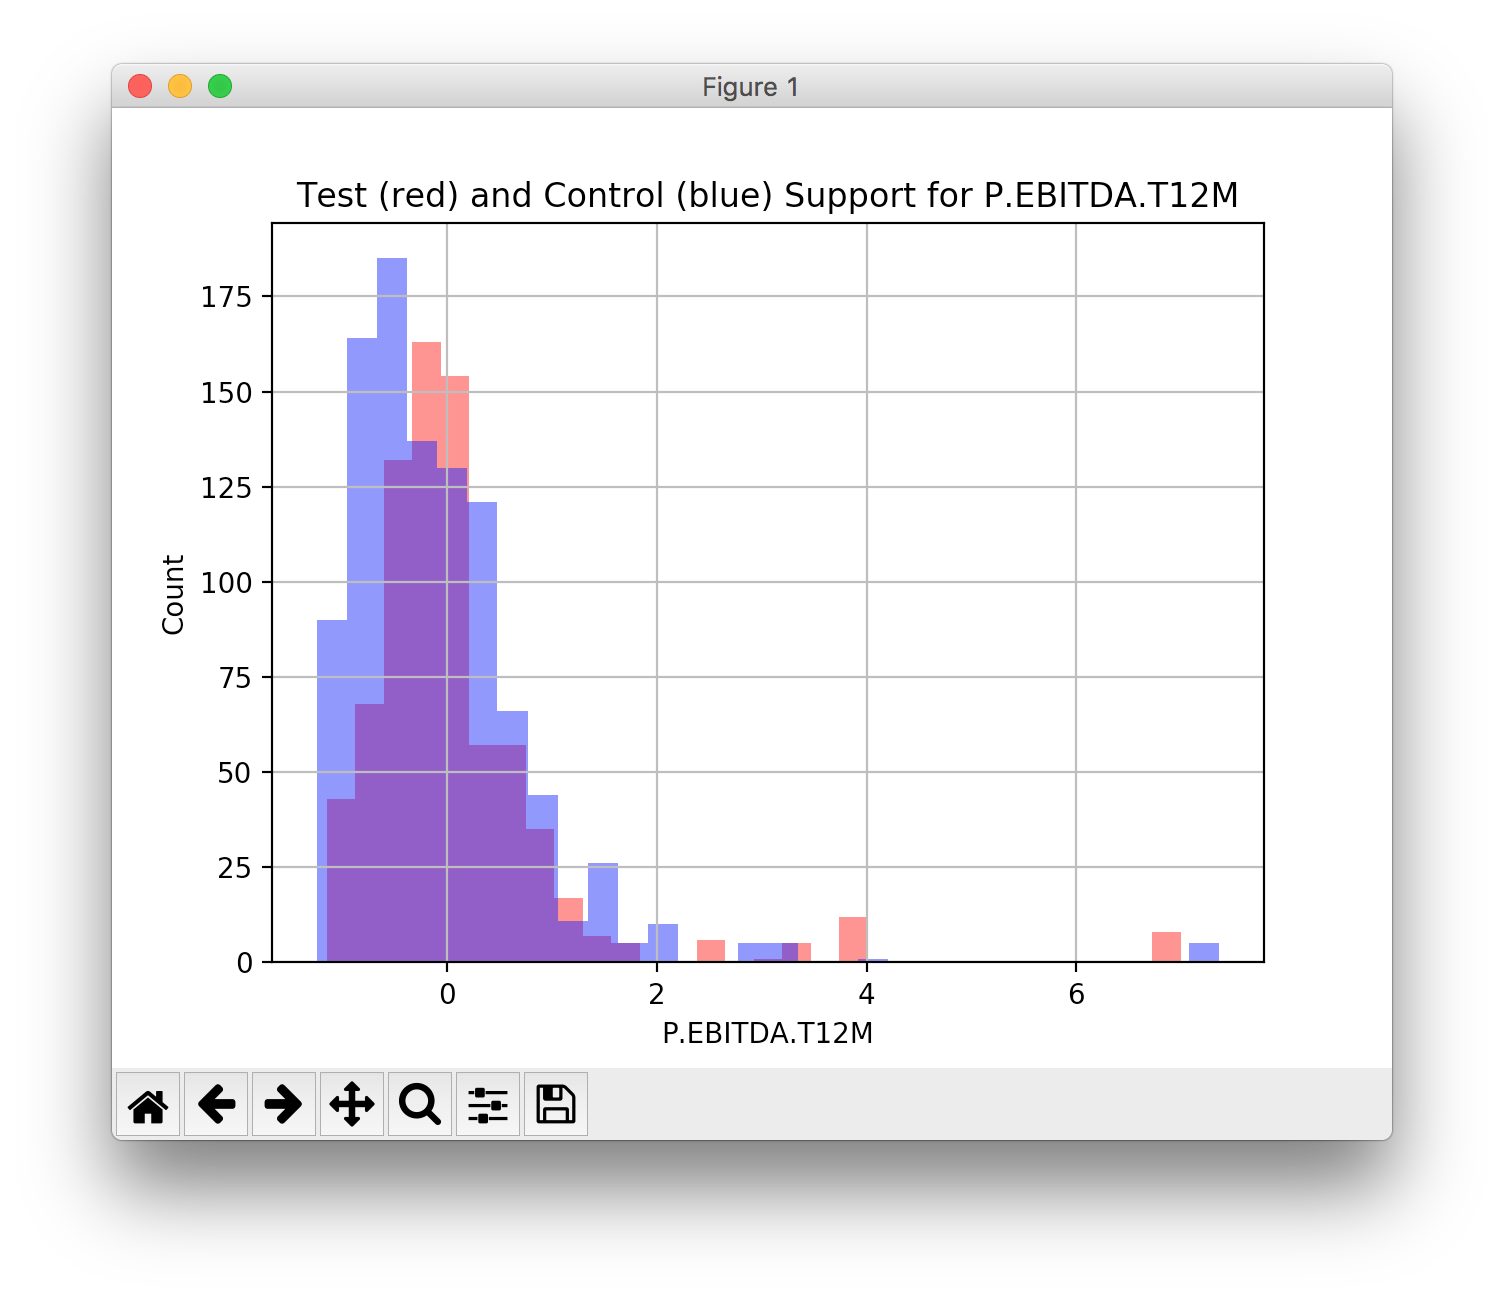
\includegraphics[width = 1.5in]{results/casual/Indep_Chrprsn_Feml_CEO_or_Equiv/altman/P_EBITDA_T12M.png}}  &
\subfigure[caption]{\includegraphics[width = 1.5in]{results/casual/Indep_Chrprsn_Feml_CEO_or_Equiv/altman/PE.png}} 
\end{tabular}
\caption{Indep\_Chrprsn\_Feml\_CEO\_or\_Equiv / Altman Z}
\end{figure}
{\bf Interval: } {(0.020997659295183047, 0.044777526679613475, 0.068637425725528167) }
\clearpage


\subsection{CEOPayOverMedian - SPX}
\begin{figure}[h!]
\begin{tabular}{ccc}
\subfigure[caption]{\includegraphics[width = 1.5in]{results/casual/CEOPayOverMedian/tobin/Asset.png}} &
\subfigure[caption]{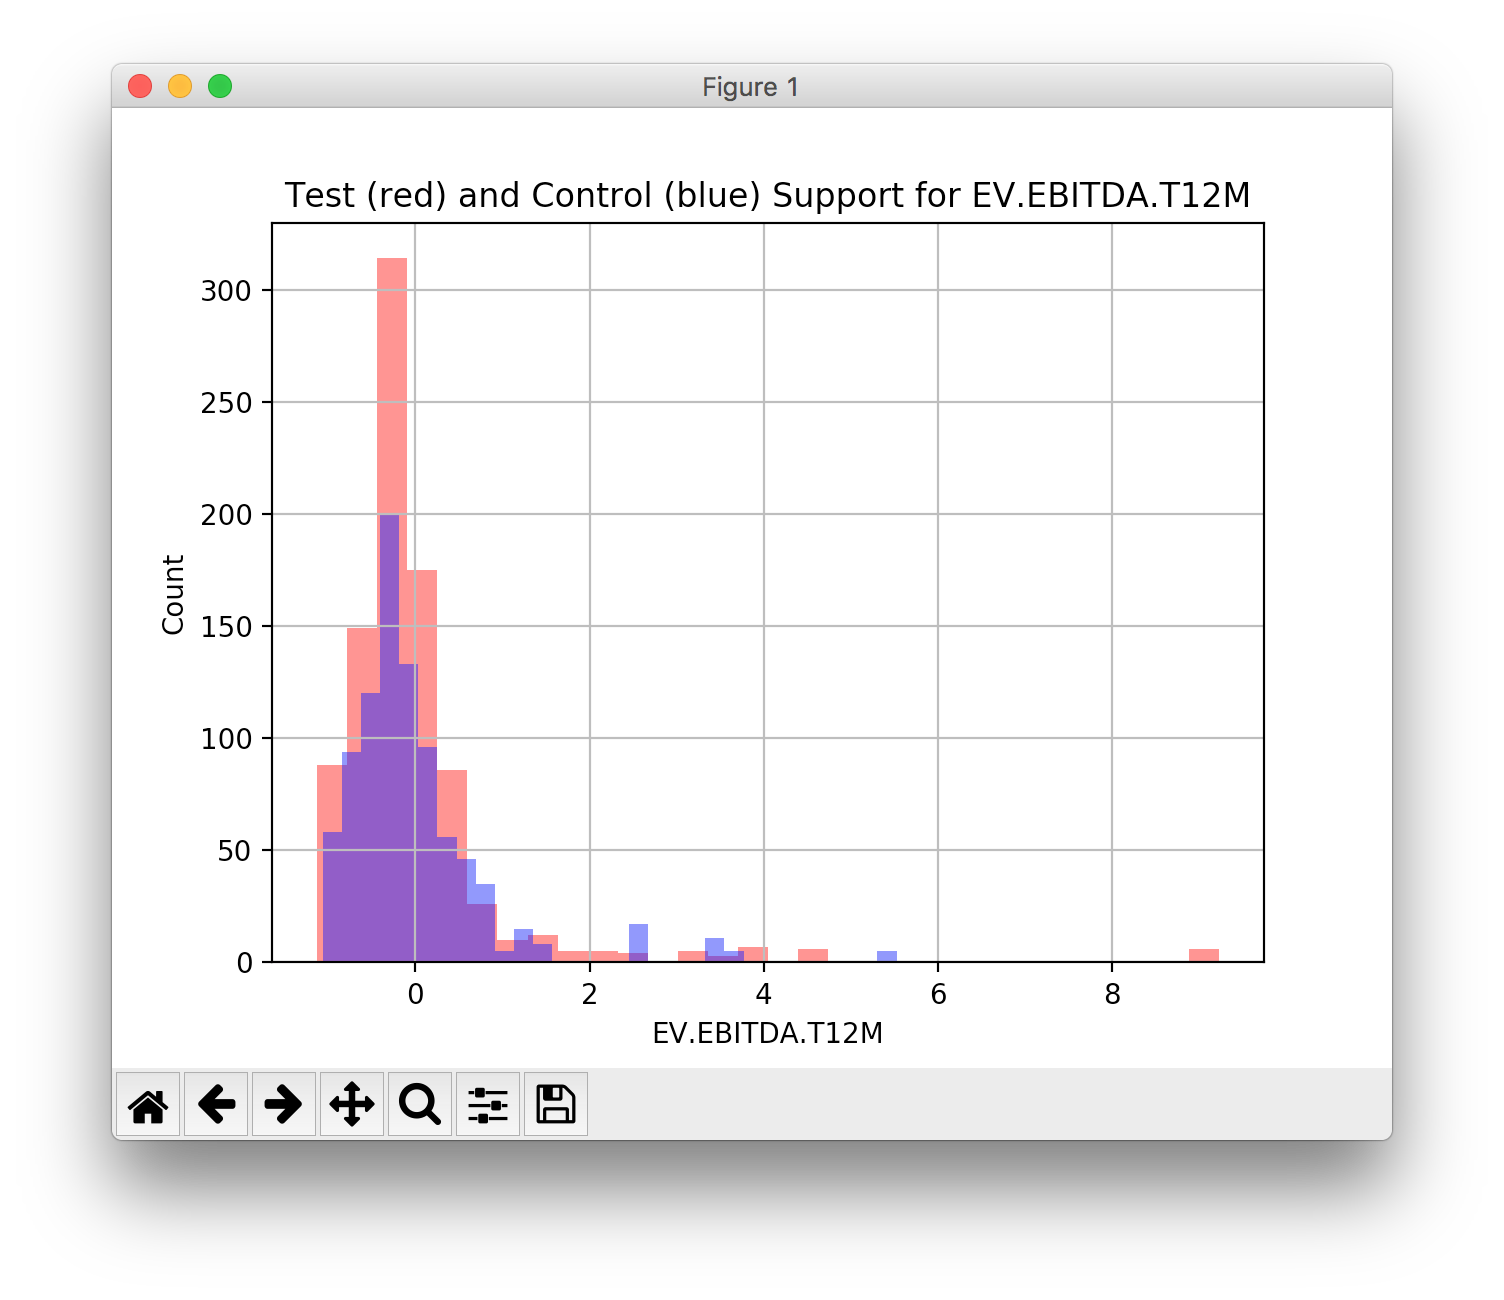
\includegraphics[width = 1.5in]{results/casual/CEOPayOverMedian/tobin/EV_EBITDA_T12M.png}} &
\subfigure[caption]{\includegraphics[width = 1.5in]{results/casual/CEOPayOverMedian/tobin/Fincl.png}} \\
\subfigure[caption]{\includegraphics[width = 1.5in]{results/casual/CEOPayOverMedian/tobin/Net_Debt_to_EBITDA.png}} &
\subfigure[caption]{\includegraphics[width = 1.5in]{results/casual/CEOPayOverMedian/tobin/Norm_NI_to_NI_for_Cmn.png}} &
\subfigure[caption]{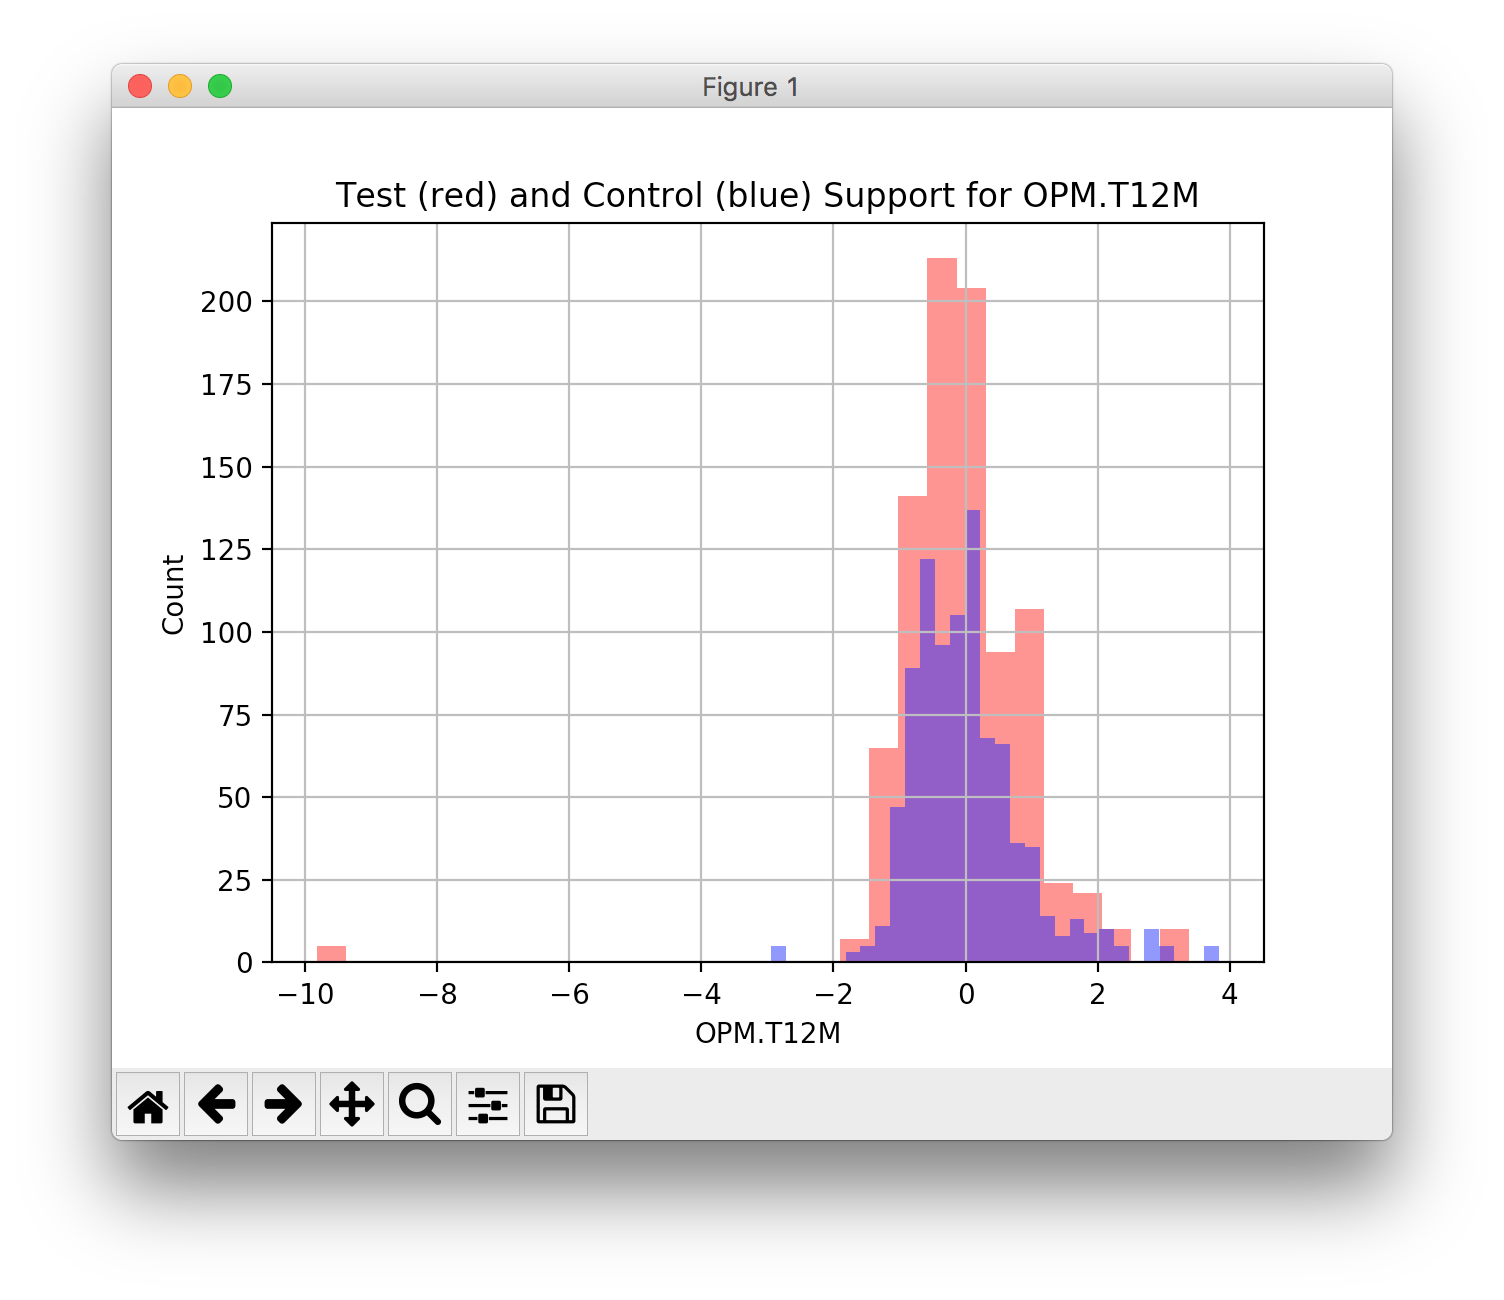
\includegraphics[width = 1.5in]{results/casual/CEOPayOverMedian/tobin/OPM_T12M.png}} \\
\subfigure[caption]{\includegraphics[width = 1.5in]{results/casual/CEOPayOverMedian/tobin/P_B.png}}  &
\subfigure[caption]{\includegraphics[width = 1.5in]{results/casual/CEOPayOverMedian/tobin/P_EBITDA.png}}  &
\subfigure[caption]{\includegraphics[width = 1.5in]{results/casual/CEOPayOverMedian/tobin/ROC.png}} \\
\subfigure[caption]{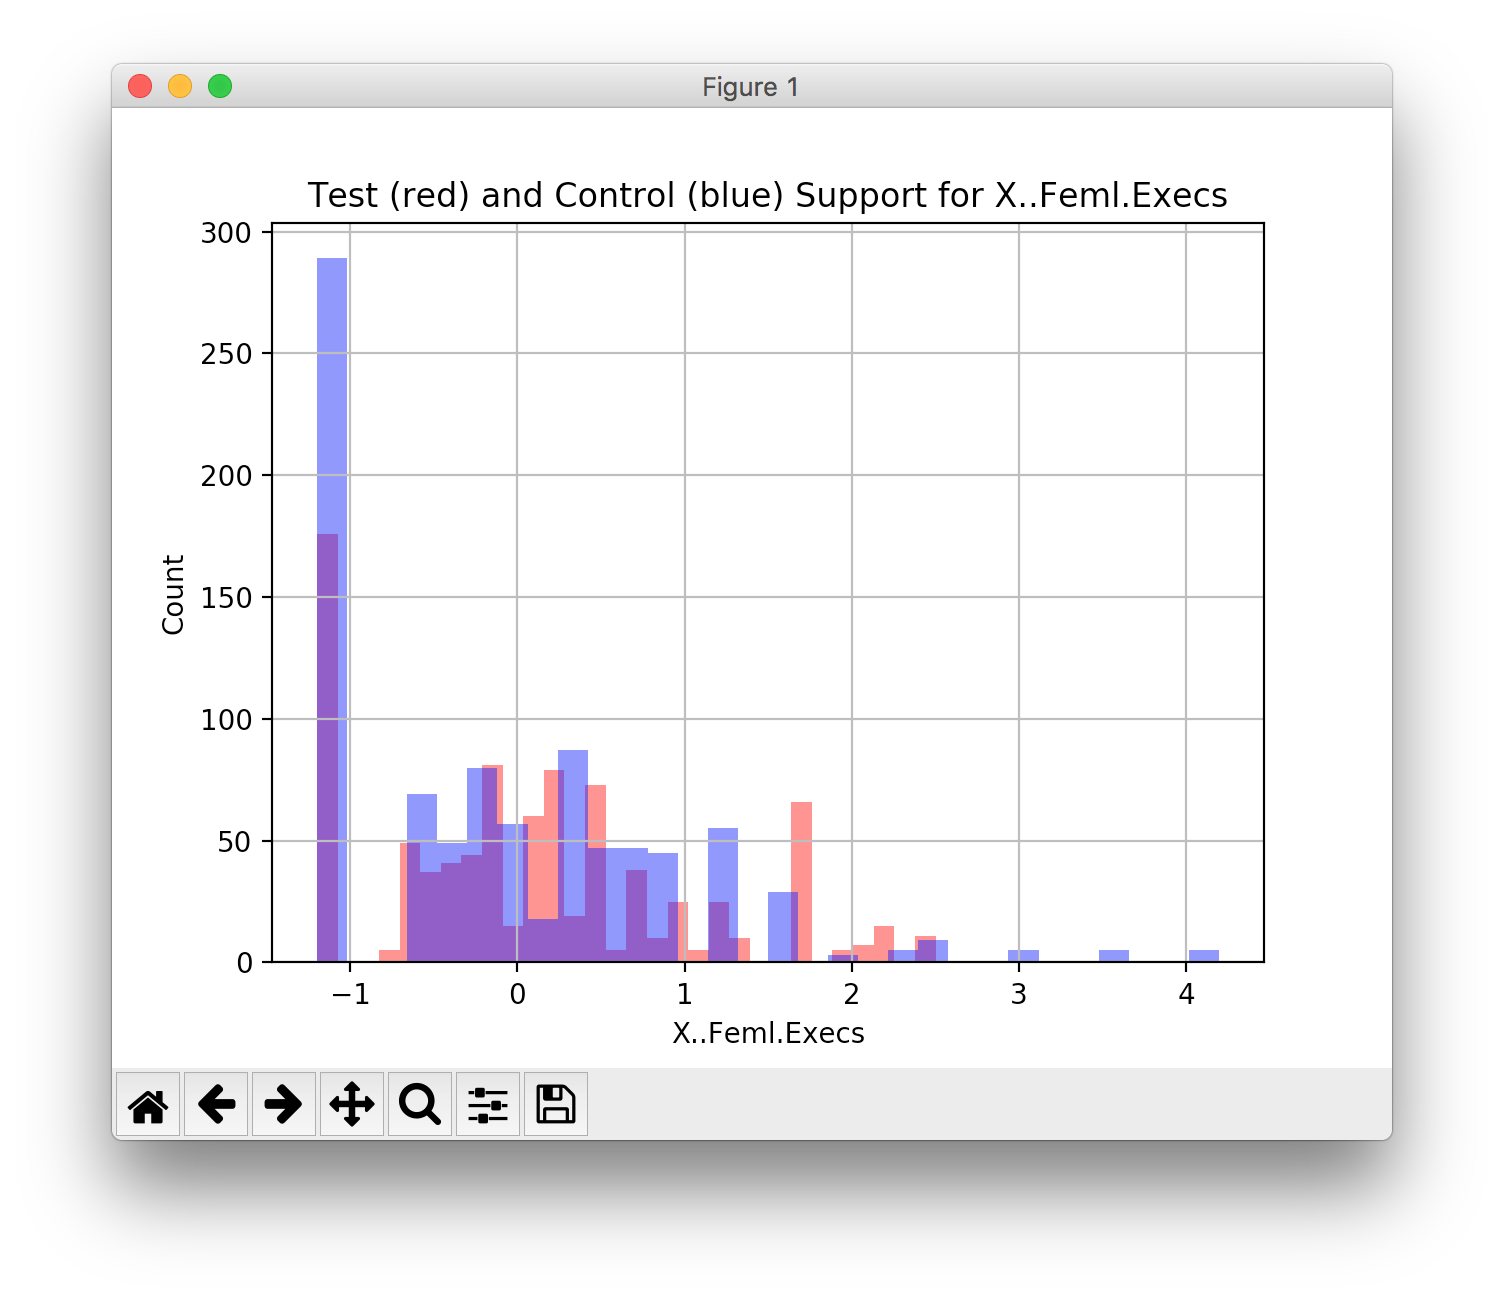
\includegraphics[width = 1.5in]{results/casual/CEOPayOverMedian/tobin/X_Feml_Execs.png}}  
\end{tabular}
\caption{CEOPayOverMedian / Tobins Q}
\end{figure}
{\bf Interval: } {(-0.090223477054923285, -0.06532611996489217, -0.040146099747952961)}
\clearpage

\begin{figure}[h!]
\begin{tabular}{ccc}
\subfigure[caption]{\includegraphics[width = 1.5in]{results/casual/CEOPayOverMedian/altman/Asset.png}} &
\subfigure[caption]{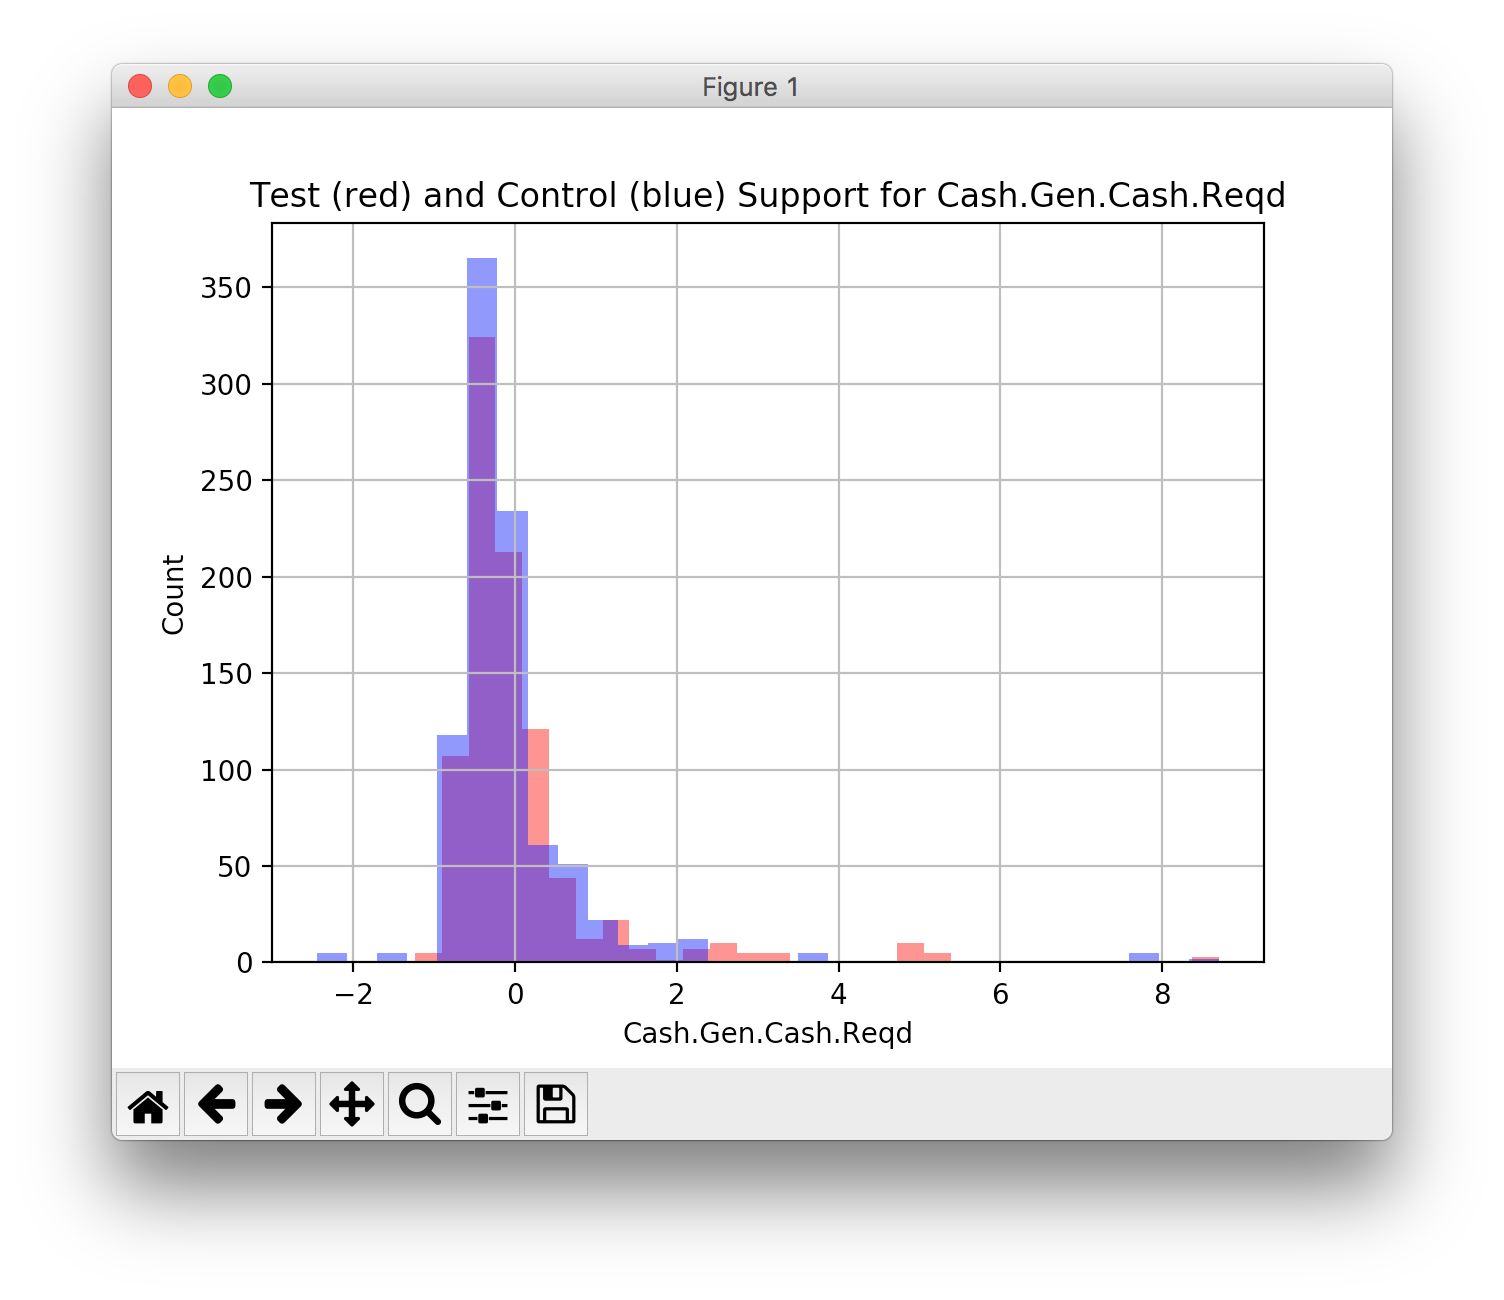
\includegraphics[width = 1.5in]{results/casual/CEOPayOverMedian/altman/Cash_Gen_Cash_Reqd.png}} &
\subfigure[caption]{\includegraphics[width = 1.5in]{results/casual/CEOPayOverMedian/altman/Fincl.png}} \\
\subfigure[caption]{\includegraphics[width = 1.5in]{results/casual/CEOPayOverMedian/altman/Net_Debt_to_EBITDA.png}} &
\subfigure[caption]{\includegraphics[width = 1.5in]{results/casual/CEOPayOverMedian/altman/Norm_NI_to_NI_for_Cmn.png}} &
\subfigure[caption]{\includegraphics[width = 1.5in]{results/casual/CEOPayOverMedian/altman/P_B.png}} \\
\subfigure[caption]{\includegraphics[width = 1.5in]{results/casual/CEOPayOverMedian/altman/P_EBITDA.png}}  &
\subfigure[caption]{\includegraphics[width = 1.5in]{results/casual/CEOPayOverMedian/altman/ROC.png}}  &
\subfigure[caption]{\includegraphics[width = 1.5in]{results/casual/CEOPayOverMedian/altman/Tax.png}} \\
\subfigure[caption]{\includegraphics[width = 1.5in]{results/casual/CEOPayOverMedian/altman/X5Yr_Avg_Adj_ROE.png}}  
\end{tabular}
\caption{CEOPayOverMedian / Altman Z}
\end{figure}
{\bf Interval: } {(-0.055123647006892637, -0.03307470810522401, -0.0064863255004465239)}



